\documentclass{book}
\usepackage{M.1.0.0}
\usepackage{listings}
\newcommand{\specialcell}[2][c]{%
  \begin{tabular}[#1]{@{}c@{}}#2\end{tabular}}

%  % % % % % % % % % % % % % % % % % % % % % % % % % % % % % % % % % % % %
%
%                                                                 INICIO DEL DOCUMENTO 
% % % % % % % % % % % % % % % % % % % % % % % % % % % % % % % % % % % % %

%  % % % % % % % % % % % % % % % % % % % % % % % % % % % % % % % % % % % %
\begin{document}

\Ini

\tableofcontents 

\Figura

\Cuadros


\Res{Resumen}
                  
El objetivo del m\'odulo de f\'isica de este megaproyecto fue caracterizar las se\~nales obtenidas del detector con una simulaci\'on Monte Carlo y calibrar el detector a trav\'es del modo histograma. Se utilizaron el sistema de adquisici\'on ACQUA, la \textit{suite} de an\'alisis ANNA de LAGO y programas propios para obtener y analizar los datos del detector. Se encontr\'o el valor VEM para Kinich Ahau, de (250 $\pm$ 20) ADCq, con el que se clasifican los eventos por bandas por el modo histograma. La simulaci\'on del detector se realiz\'o con Geant4, y se determin\'o que la cantidad de fotones detectados en la simulaci\'on Geant4 generados por muones con energ\'ias suficientes para atravesar el tanque depende de la energ\'ia de los muones, con una correlaci\'on de 10.3 $GeV^{-1}$ y un valor p de 0.006 para la regresi\'on lineal. Se caracteriz\'o las se\~nales de pulsos t\'ipicos del experimento con la simulaci\'on Geant4, obteniendo las amplitudes y tiempos de subida promedio de tres tipos de evento: muones de 4GeV que logran atravesar el tanque, part\'iculas gamma de 100 MeV que producen pares cargados y electrones con energ\'ias t\'ipicas de la distribuci\'on de Michael en el decaimiento de un mu\'on.

\Chapter{Introducci\'on}
\UnoA

El presente Megaproyecto tiene como objetivo dise\~nar y construir un detector de radiaci\'on Cherenkov de agua (WCD por sus siglas en ingl\'es) para tomar y procesar datos en la determinaci\'on de eventos atmosf\'ericos como consecuencia de reducci\'on Forbush. Al culminar la realizaci\'on de este proyecto se pretende promover un intercambio generacional de conocimientos de part\'iculas de altas energ\'ias, contribuir el \'area de investigaci\'on de este tipo en Guatemala, colaborar con la recopilaci\'on de informaci\'on por parte de observatorios LAGO, y servir como referencia para la construcci\'on de observatorios similares a mayores altitudes en otras regiones del pa\'is.

El presente proyecto no es capaz de determinar la direcci\'on de incidencia de las part\'iculas secundarias. Esto se debe a que la informaci\'on de esta direcci\'on se pierde durante la captura de fotones \'opticos dentro del tanque; es decir, esta captura de fotones no es suficientemente r\'apida y eficiente como para reconstruir informaci\'on sobre la direcci\'on de la part\'icula incidente. El proyecto tampoco es capaz de detectar rayos gamma, ya que el tanque no es suficientemente alto para que ocurra producci\'on de pares y tambi\'en porque el flujo disminuye considerablemente entre menor altitud: la Ciudad de Guatemala est\'a a una altitud media de 1500 metros sobre el nivel del mar. Tampoco puede recobrar informaci\'on significativa sobre part\'iculas primarias de las cascadas extensas de rayos c\'osmicos, nuevamente, por la baja altitud e insuficiente \'area superficial del detector.

El m\'odulo de f\'isica en este megaproyecto abarca la caracterizaci\'on de se\~nal de eventos. Esto incluye la elaboraci\'on de una simulaci\'on Monte Carlo de eventos en el tanque y la elaboraci\'on de estrategias para la calibraci\'on de datos y la identificaci\'on de part\'iculas a partir de la se\~nal de eventos. La simulaci\'on Monte Carlo tiene como objetivo caracterizar el conteo de fotones por el fotomultiplicador para el evento de un mu\'on o gamma secundario, y se realiz\'o utilizando la herramienta GEANT4 desarrollada por CERN. El resultado de esta simulaci\'on es una completa descripci\'on de la forma esperada de la se\~nal en el fotomultiplicador para un evento t\'ipico de mu\'on que atravieza el tanque, mu\'on que decae y el electr\'on que produce, y rayos gamma que producen pares, y esto para diferentes \'angulos de incidencia y a lo largo del espectro de energ\'etico de un mu\'on o rayo gamma como part\'icula secundaria proveniente de una cascada extensa.

\Chapter{Objetivos}

\section{Objetivo general del megaproyecto}
Dise\~nar y construir un detector de radiaci\'on Cherenkov de agua para tomar y procesar datos, en la identificaci\'on de part\'iculas secundarias provenientes de cascadas extensas de rayos c\'osmicos inciden en el detector de radiaci\'on Cherenkov de agua.
\section{Objetivo general del m\'odulo}
Caracterizar las se\~nales obtenidas del detector utilizando el modo histograma y con una simulaci\'on Monte Carlo utilizando Geant4.
\section{Objetivos espec\'ificos}
\begin{itemize}
 \item Obtener la calibraci\'on por el mu\'on vertical equivalente (VEM) del an\'alisis de primer nivel de los datos de ACQUA del montaje experimental en el tanque.
 \item Calcular la vida media del mu\'on a partir de una corrida del experimento en el WCD.
 \item Obtener la forma representativa de pulsos en el tiempo con la simulaci\'on en geant4 para muones que atraviesan, muones que decaen, electrones, sus antipart\'iculas respectivas, y part\'iculas gamma.
\end{itemize}

%%%%%%%%%%%%%%%%Cap\'itulo nuevo

\Chapter{Justificaci\'on}

El detector construido en este megaproyecto es cap\'as de realizar mediciones indirectas de la modulaci\'on de heli\'osfera de los rayos c\'osmicos. Por lo tanto, es una herramienta viable para el monitoreo de la actividd solar. Debido a que la actividad solar y eventos en el medio interplanetario tienen efectos disruptivos sobre la magnet\'osfera, el estudio del efecto de fen\'omenos solares desde diferentes posiciones en la Tierra es muy valioso para prevenir da\~nos sobre sat\'elites y problemas en transmisiones de radio. Esto es cada vez m\'as importante debido a la progresiva sofisticaci\'on de los aparatos electr\'onicos.

Por otro lado, este es uno de los pocos proyectos de f\'isica experimental en Guatemala, por lo que su valor formativo en el trabajo cient\'ifico en la comunidad es importante ya que establece una plataforma para continuar la investigaci\'on de part\'iculas de altas energ\'ias de origen astrof\'isico. El intercambio generacional que originar\'a el proyecto, as\'i como su mantenimiento y replicaci\'on ser\'an formativos para estudiantes de f\'isica, qu\'imica e ingenier\'ias. Adem\'as, el trabajo en la electr\'onica de instrumentaci\'on del proyecto ser\'a un gran avance en el desarrollo tecnol\'ogico del pa\'is.

%%%%%%%%%%%%%%%%Cap\'itulo nuevo

\Chapter{Rayos c\'osmicos}
\section{Generalidades y descubrimiento de los rayos c\'osmicos}
Los rayos c\'osmicos (RC) son part\'iculas que se originan fuera del Sistema Solar y llegan a la Tierra o su entorno cercano, excluyendo a los fotones. Generalmente estas part\'iculas son n\'ucleos at\'omicos, desde hidr\'ogeno hasta de hierro. Se les denomina tambi\'en \textit{primarios}, especialmente en el contexto de cascadas de \'area extensa (descritas en la secci\'on 4.5). Los rayos c\'osmicos fueron descubiertos porque en laboratorios de f\'isica se observaba que electr\'ometros cargados y aislados de fuentes radioactivas se descargaban sin aparente raz\'on, y la mejor explicaci\'on que se encontr\'o para este fen\'omeno era el flujo extraterrestre de part\'iculas de altas energ\'ias. \citep{ASOREY}

Theodor Wulf desarroll\'o a los inicios del siglo XX un electroscopio m\'as sensible que los de su \'epoca y not\'o que en la punta de la Torre Eiffel la tasa de decaimiento era mayor de la esperada tomando en cuenta \'unicamente la radiaci\'on gamma, que era la \'unica fuente relevante considerada para esa situaci\'on. Por otro lado, Domenico Pacini, realiz\'o tres mediciones: a nivel del suelo, en la superficie del Lago Bracciano, y a tres metros de profundidad en el lago. Comparando estas mediciones, en las que se destacaba que bajo el agua la tasa disminu\'ia, concluy\'o que debe de haber una fuente de radiaci\'on adicional. \citep{ASOREY}

V.F. Hess en 1912 fue quien finalmente dijo que la fuente de esta radiaci\'on es de origen extraterrestre y que ingresa desde arriba de la atm\'osfera con gran poder penetrante. El experimento que realiz\'o le gan\'o el Nobel de F\'isica en 1936. Consist\'ia en la medici\'on de tasas de ionizaci\'on a diferentes altitudes. Las mediciones las realiz\'o durante 10 vuelos en globos aereost\'aticos hasta los 5000 m.s.n.m. La dependencia de la tasa de ionizaci\'on sobre la altitud fue lo que llev\'o a su importante conclusi\'on. \citep{ASOREY}

Los rayos c\'osmicos tienen un rango de energ\'ia extremadamente amplio: desde $10^5 eV$, que incluye part\'iculas del viento solar hasta $10^{20} eV$, part\'iculas intergal\'acticas. Los rayos c\'osmicos de ultra alta energ\'ia son primarios con energ\'ias superiores a $E_p \geq 10^{18} eV$. Su medici\'on directa es casi imposible debido al baj\'isimo flujo. En cambio, se infiere su existencia por la detecci\'on de las part\'iculas secundarias producidos por la cascada de \'area extensa generada por el ingreso del primario. Esto fue observado por primera vez en 1934 por Bruno Rossi quien not\'o que equipos separados por gran distancia detectaban simult\'aneamente aumentos en el conteo de part\'iculas; Pierre Auger infiri\'o en 1938 que esto era explicado por el ingreso de una part\'icula primaria de energ\'ias superiores a los $10^{15}eV$. \citep{ASOREY}

\section{Or\'igenes de los rayos c\'osmicos de ultra alta energ\'ia}

La explicaci\'on de rayos c\'osmicos de ultra alta energ\'ia es todav\'ia un problema abierto. Los modelos de aceleraci\'on proponen que estas part\'iculas pueden alcanzar energ\'ias tan altas por el efecto de aceleradores naturales en el universo. Un mecanismo de aceleraci\'on es cuando rayos c\'osmicos atraviesan una nube de gas en el medio interplanetario. El efecto de esta interacci\'on es un aumento en la energ\'ia del RC. Sin embargo, este aumento es ineficiente a menos que la velocidad propia de la nube sea de magnitudes relativistas ($\beta\approx1$). Un ejemplo de material que cumple con esto son los frentes de choque producidos por supernovas, que s\'i podr\'ian explicar grandes aceleraciones. Sin embargo, estos modelos sufren a\'un de sobresimplificaci\'on, ya que consideran la densidad en los frentes de choque como funciones escal\'on y que el frente es no relativista.\citep{ASOREY}

Otra explicaci\'on de los rayos c\'osmicos de ultra alta energ\'ia son fuentes con intensos campos magn\'eticos y grandes dimensiones. Fuentes extragal\'acticas de rayos c\'osmicos podr\'ian ser los n\'ucleos gal\'acticos activos, blazares y p\'ulsares son posibles candidatos. Una limitante a esta idea es el corte GZK, que es el l\'imite te\'orico para la energ\'ia de rayos c\'osmicos extragal\'acticos. El l\'imite lo establece el hecho de que rayos c\'osmicos que atraviesan grandes distancias interact\'uan con el fondo c\'osmico de microondas, perdiendo energ\'ia. Los RC provenientes de estas fuentes estar\'ian viajando desde un universo isotr\'o por lo que la distribuci\'on que los detectores observar\'ian ser\'ia isotr\'opica. En cambio, si las fuentes de aceleraci\'on de rayos c\'osmicos de ultra alta energ\'ia est\'an dentro de la galaxia, como en los modelos de aceleraci\'on mencionados anteriormente, la distribuci\'on de la direcci\'on de los RC apuntar\'ia a estas fuentes. Esto puntualiza la importancia de proyectos de detectores terrestres que sean capaces de determinar la direcci\'on de arribo de RC, ya que dar\'ian m\'as peso a una explicaci\'on que la otra. \citep{PEREZ}

\section{Modulaci\'on solar de rayos c\'osmicos}

La traves\'ia de los rayos c\'osmicos es afectada por el campo magn\'etico en el espacio. Cuando los rayos c\'osmicos entran al sistema solar, se encuentran con el campo magn\'etico interplanetario producido por el Sol. Cuando ocurren eventos como eyecciones de masa coronal, el campo magn\'etico interplanetario se intensifica y los rayos c\'osmicos son desviados. Estos fen\'omenos consisten en la variaci\'on r\'apida del flujo de rayos c\'osmicos en la superficie terrestre, seguida por una eyecci\'on coronal desde el Sol, llamados decrecimientos Forbush. Este efecto fue descubierto por Scott E. Forbush en 1937, que tambi\'en observ\'o que la intensidad de los RC al alcanzar la Tierra se encontraban inversamente correlacionados con los 11 a\~nos de ciclo solar de las manchas solares. Un detector que lleve la cuenta permanente de los rayos c\'osmicos que llegan a tierra puede dar informaci\'on acerca de estos eventos solares que originan los decrecimientos Forbush. A partir de los datos “residuales” de los tanques de agua del Pierre Auger, han construido un an\'alisis de modulaciones solares de rayos c\'osmicos -en los que entran los Forbush decreases- y los compararon con los mismos an\'alisis para estos eventos estudiados en detectores de neutrones, concluyendo que es un estudio valioso, viable, y complementario en especial a las mediciones por sondas espaciales “in situ” que recolectan esa info en el espacio; el an\'alisis de rayos c\'osmicos desde el suelo es complementario porque puede dar informaci\'on de la estructura de la heli\'osfera y de ICME (interplanetary corona mass ejection), ya que la capacidad de las sondas de hacer esto es m\'inima. \citep{VILLASENOR}

\begin{figure}[ht] %opci\'on h - here pone la imagen aqu\'i en esta posici\'on del documento
\begin{center}
 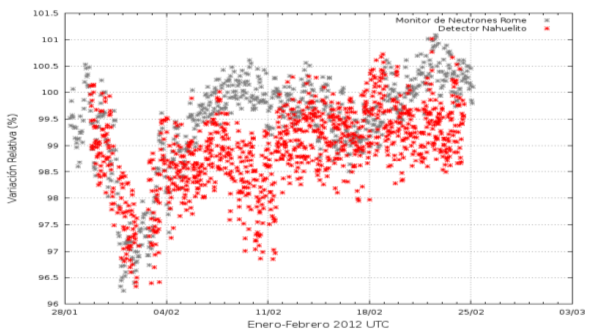
\includegraphics[width = 0.7\linewidth]{ForbushYunior.png}
 
 Extra\'ido de \citep{PEREZ}
\caption{Conteo en el detector Nahuelito durante un decrecimiento Forbush entre enero y febrero, graficado junto al conteo por el monitor de neutrones Rome}
\end{center}
\end{figure}

\section{Cascadas de \'area extensa de rayos c\'osmicos}
Una cascada de \'area extensa (CAE) es la lluvia de part\'iculas originada por la interacci\'on de un rayo c\'osmico con un n\'ucleo de elemento constituyente de la atm\'osfera. Lo que determina la forma de la cascada es la cantidad de materia atravesada, por lo que la densidad (y, por ende, la presi\'on atmosf\'erica) tiene una influencia directa sobre el flujo de part\'iculas en el suelo. Esta anticorrelaci\'on entre presi\'on atmosf\'erica y flujo debe de ser corregida si se quiere obtener informaci\'on sobre el flujo de part\'iculas. En el estudio de las CAE, se define la profundidad atmosf\'erica $X(l)$ como la masa de aire por unidad de \'area que atraviesa la part\'icula desde el infinito hasta la posici\'on $l$,

\begin{equation}
X(l)=\int_{l}^{\inf}\rho(l)dl
\end{equation}

Donde, adem\'as, $\rho(l)$ est\'a dada por la ecuaci\'on barom\'etrica para la densidad atmosf\'erica con una temperatura $T(h)$

\begin{equation}
\rho(h)=\rho(h_0)\Bigg(\frac{T(h_0)}{T(h)}\Bigg)exp\Bigg(-\int_{h_0}^{h}\frac{M}{R}\frac{g(h)}{T(h)}dh\Bigg)
\end{equation}

siendo $R$ la constante universal de los gases, $M$ la masa molar del aire y $g(h)$ la aceleraci\'on debido a la gravedad a una altura $h$. Por construcci\'on, el valor $X(0)$ se obtiene directamente de la presi\'on atmosf\'erica a nivel del mar con $P_0/g_0=101325Pa/9.81ms^{-2}=1033gcm^{-2}$ \citep{YUNIOR}

\begin{figure}[ht] %opci\'on h - here pone la imagen aqu\'i en esta posici\'on del documento
\begin{center}
 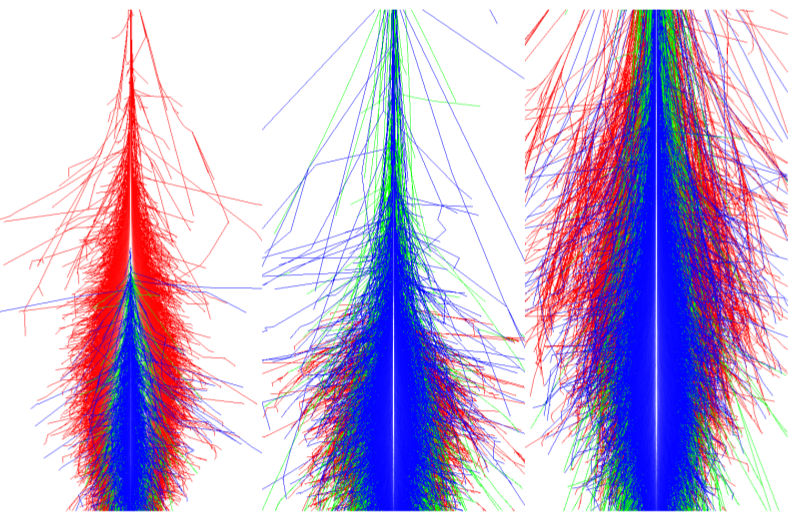
\includegraphics[width = 0.7\linewidth]{Cascadas.png}
 
 Extra\'ido de \citep{ASOREY}
\caption{Desarrollo longitudinal y lateral de cascadas de \'area extensa producidas por un fot\'on (izquierda), un prot\'on (centro) y un \'atomo de hierro (derecha). Los colores indican las tres cascadas principales: la parte electromagn\'etica (rojo), mu\'onica (verde) y hadr\'onica (azul).}
\end{center}
\end{figure}

La distribuci\'on lateral al eje de la lluvia tiene un m\'aximo en alg\'un lugar sobre el nivel del mar, t\'ipicamente entre 4 y 7 km. Luego de este punto de mayor radio de la cascada, la creaci\'on de part\'iculas secundarias disminuye y la densidad de part\'iculas tambi\'en. Se caracteriza la edad de la cascada (S) alrededor de este punto m\'aximo (S$<$1 para antes de ese m\'aximo, S=1 cuando ocurre ese m\'aximo y S$>$1 para luego del m\'aximo). \citep{ASOREY}\citep{SUAREZ}

Una cascada lleva a tres componentes: electromagn\'etico, de muones y de hadrones; 1\% es de hadrones, 10\% son muones y 89\% son part\'iculas cargadas (electrones y positrones). El 90\% de la energ\'ia est\'a en el canal electromagn\'etico. El n\'umero total de part\'iculas secundarias depende de a) la energ\'ia de la part\'icula primaria (12-20 \'ordenes de magnitud eV) b) \'angulo cenital (entre $0^o$, vertical, y $90^o$, horizontal), c) punto de primer interacci\'on. El \'angulo cenital influye en gran medida, porque una part\'icula que ingresa a la atm\'osfera con un \'angulo cercano a 90 grados tiene una cascada sobre el suelo 40 veces menos energ\'etica que una que entr\'o verticalmente. El primer punto de interacci\'on depende adem\'as del tipo de part\'icula primaria. \citep{ASOREY}\citep{SUAREZ}

\subsection{Distribuci\'on de energ\'ias a nivel del suelo}
Para observatorios de Cherenkov en agua, es importante conocer la distribuci\'on de energ\'ia de muones ya que los de energ\'ias mayores a 0.3 GeV son los que atraviesan los tanques y se usan para calibraci\'on. Otro tipo de part\'icula que alcanzan detectores son los rayos gamma de 100 MeV, sin embargo, el flujo de rayos gamma disminuye luego del m\'aximo de la cascada as\'i que \'unicamente detectores de gran altitud los detectan apreciablemente. \citep{WATSON}

La f\'ormula est\'andar de Geisser describe la distribuci\'on energ\'etica de muones a nivel del suelo cuando la curvatura de la Tierra puede ser obviada y cuando el decaimiento de muones es negligible. Estas condiciones son equivalentes a tomar \'unicamente eventos con \'angulo cenitar menor a 70 grados y considerar muones con energ\'ias mayores a $100/\cos\theta GeV$. Sin embargo, la mayor\'ia de muones encontradas a nivel del suelo tienen energ\'ias menores a este l\'mite. El trabajo de Guan et al. extiende la f\'ormula de Geisser agreg\'ando par\'ametros ajustados por datos experimentales. La distribuci\'on energ\'etica dada es entonces

\begin{equation}
\frac{dN}{dE}=p_{0}0.14E^{-2.7}\Bigg[\frac{115}{1.1E}ln\Bigg[\frac{1+\frac{1.1E}{115}}{1+0.342\frac{1.1E}{115}}\Bigg]+\frac{45.9}{1.1E}ln\Bigg[\frac{1+\frac{1.1E}{850}}{1+0.342\frac{1.1E}{850}}\Bigg]\Bigg]
\end{equation}

donde $\theta$ es el \'angulo polar y $E$ es la energ\'ia en $GeV$. Esta f\'ormula representa la distribuci\'on de muones de cascadas extensas a nivel del suelo. Los par\'ametros mencionados se ajustaron usando CORSIKA usando una densidad atmosf\'erica de $114.8 g/cm^3$. La figura 4.1 muestra esta distribuci\'on. Un ajuste de potencia a esta gr\'afica arroja la siguiente distribuci\'on \citep{GUAN}

\begin{equation}
d(E)=(4.114\pm0.003)\times10^{10}E^{-3.07143\pm0.00004}
\end{equation}

\begin{figure}[ht] %opci\'on h - here pone la imagen aqu\'i en esta posici\'on del documento
\begin{center}
 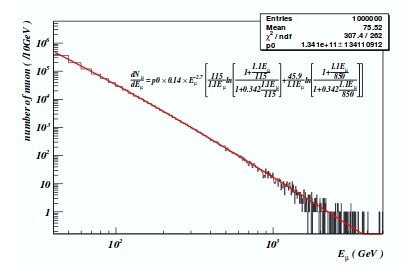
\includegraphics[width = 0.7\linewidth]{GeisserMuon.png}
 
 Extra\'ido de \citep{GUAN}
\caption{Distribuci\'on de la energ\'ia de muones generada con n\'umeros aleatorios basado en la f\'ormula de Geisser}
\end{center}
\end{figure}

\subsection{Simulaci\'on de cascadas de \'area extensa}
Para realizar simulaciones cascadas de \'area extensa se puede utilizar el programa CORSIKA, desarrollado por el Instituto de F\'isica Nuclear de Karlsruhe (IKP). \'Este simula las distintas interacciones de las part\'iculas que se generan a partir de una primera part\'icula de alta energ\'ia (part\'icula primaria) para as\'i construir la cascada. \citep{HECK}

El modelo de Heitler es un modelo simplificado que predice el comportamiento del canal electromagn\'etico de la cascada. Los dos mecanismos de interacci\'on que describe son el de frenado (Bremsstrahlung) y de pares: el primero es un electr\'on que al encontrarse con un \'atomo de la atm\'osfera desprende un electr\'on de menor energ\'ia y una part\'icula gamma, el segundo es la generaci\'on de un electr\'on y positr\'on cuando una part\'icula gamma se encuentra un \'atomo en la atm\'osfera. Estas interacciones cesan cuando la energ\'ia perdida por ionizaci\'on del electr\'on es igual a su energ\'ia en reposo (otros criterios existen para para detener el proceso dentro de una simulaci\'on). \citep{SUAREZ}

Para las interacciones hadr\'onicas de alta energ\'ia se utilizan los modelos VENUS, QGSJET, DPMJET y SIBYLL. Para las hadr\'onicas de baja energ\'ia utiliza GHEISHA. Por \'ultimo las electr\'onicas las simula con EGS4 y NKG. CORSIKA necesita que se le ingresen los siguientes datos: datos de la atm\'osfera en d\'onde se realizar\'a la simulaci\'on, el sistema coordenado a utilizar, el campo geomagn\'etico del lugar a simular y el sistema de unidades que se utilizar\'a. \citep{HECK}

\Chapter{Detectores de superficie}
La modulaci\'on solar del conteo de rayos c\'osmicos y la posibilidad de conocer los mecanismos de aceleraci\'on y producci\'on de RC delinea la importancia de la construcci\'on de detectores de las part\'iculas secundarias producidas de cascadas de \'area extensa. Como se describi\'o en el cap\'itulo 4, las primeras detecciones de rayos c\'osmicos se realizaron en el aire, en globos. En la actualidad, los  m\'etodos m\'as populares de detecci\'on son sondas en el espacio, detectores en globos, y detectores en superficie terrestre. \citep{BERN}

\section{Detectores en sondas y globos}

Algunos de los actuales experimentos en sondas y globos son
\begin{itemize}
\item Cosmic-ray Energetic and Mass (CREAM): experimentos de viajes ultra largos en globo que miden la composici\'on de rayos c\'osmicos en la escala de energ\'ias de $10^{15}$ GeV. El prop\'osito es estudiar las caracter\'isticas del espectro de rayos c\'osmicos en estas energ\'ias para establecer l\'imites a mecanismos de aceleraci\'on por supernovas. \citep{SEO}
\item Antarctic Impulsive Transient Antenna (ANITA): Circula el continente ant\'arctico a altitudes de 35-37 km. Su misi\'on es la detecci\'on de neutrinos de ultra alta energ\'ia, y logra la detecci\'on de rayos c\'osmicos de $10^{19}$ GeV. \citep{HOOVER}
\item Voyager: Su actual misi\'on es \textit{Voyager Interstellar Mission} encontr\'andose ya en la capa m\'as externa de la heli\'osfera, donde la presi\'on del gas interestelar merma los vientos solares. Estudia los campos magn\'eticos, las ondas de plasma y el flujo de part\'iculas.
\end{itemize}

\section{Detectores de superficie}

\begin{itemize}
\item Fly's-Eye y Hi-Res: El experimento Fly's-Eye oper\'o entre 1980 y 1993 en el desierto de Utah, en Estados Unidos. Era un arreglo de 67 espejos esf\'ericos de 1575 mm de di\'ametro ubicados en dos sitios separados entre s\'i, usando la t\'ecnica de fluorescencia y la separaci\'on para triangular la direcci\'on de los primarios. El experimento Hi-res fue una extensi\'on del primero, utilizando espejos m\'as grandes, y funcion\'o entre 1994 y 2006. Lograron detectar primarios de hasta $10^{20} GeV$.
\item Observatorio Pierre Auger: La instalaci\'on m\'as grande de detectores de agua de radiaci\'on Cherenkov es Pierre Auger, en Argentina. Consiste en 1660 tanques de agua dispuestos en una regi\'on triangular de 3000 kil\'ometros cuadrados, espaciados a 1500 metros. El arreglo en Pierre Auger tiene un \'area total de $16000m^{2}$ y funciona a $10^8$ conteos por minuto. Algunas especificaciones del modelo Scaler en Pierre Auger: Muestreo de 40MHz por seis 10-bit flash analog-to-digital converter (FADC), enlace de radio al CDAS (central data acquisition system), sistema GPS para sincronizar los 1660 tanques. La respuesta del detector est\'a hecha para el resultado de un conjunto de simulaciones de cascadas de baja energ\'ia usando CORSIKA 6.980 modelo QGSJET-II para hadrones alta energ\'ia y GHEISHA para bajas. El flujo de part\'iculas primarias a 100 km se simula como una ley de poder, cuyo exponente se obtuvo de mediciones de espectro de energ\'ias de la part\'icula primaria. \citep{VILLASENOR}
\end{itemize}

\section{Radiaci\'on de Vavilov-Cherenkov}
Una part\'icula cargada movi\'endose en un material puede polarizar los \'atomos que la circundan ya que su campo magn\'etico en ese instante y en ese lugar distorsiona a los \'atomos induciendo sus dipolos el\'ectricos. Esta polarizaci\'on es moment\'anea y local, ya que cuando la part\'icula cargada se aleja, los \'atomos retornan a su forma normal. Debido a la simetr\'ia de la polarizaci\'on alrededor de la carga, el campo magn\'etico desaparece lejos de la part\'icula y no ocurre radiaci\'on (figura 5.1.a). \citep{PEREZ}

\begin{figure}[ht] %opci\'on h - here pone la imagen aqu\'i en esta posici\'on del documento
\begin{center}
 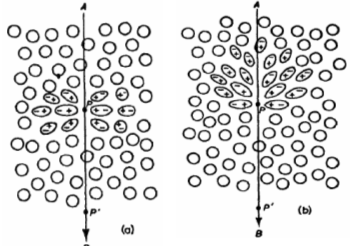
\includegraphics[width = 0.5\linewidth]{Pol1.png}
 
 Extra\'ido de \citep{GROUPENS}
\caption{a) paso de una part\'icula cargada en un medio transparente con velocidades bajas. b) paso de una part\'icula cargada en un material transparente con velocidad mayor a la velocidad de la luz en ese material}
\end{center}
\end{figure}

La simetr\'ia mencionada se rompe si la part\'icula cargada se mueve a una velocidad mayor a la velocidad de la luz en ese medio (figura 5.1.b). Es decir,

\begin{equation}
\beta > \frac{1}{n}
\end{equation}

donde $\beta$ se refiere a la part\'icula incidente y $n$ es el \'indice de refracci\'on del material. En este caso, las ondas radiadas por el paso de la carga produce interferencia constructiva a ciertas posiciones respecto a la carga. Dado un tiempo $t$, la coherencia en la onda est\'a delimitada por la distancias que la luz y la part\'icula recorren en ese tiempo, como mostrado en la figura 5.2. La distancia que recorre la luz ser\'ia $ct/n$ y la que recorre la part\'icula ser\'ia $\beta ct$. El \'angulo $\theta_c$ formado se relaciona con esas distancias por

\begin{figure}[ht] %opci\'on h - here pone la imagen aqu\'i en esta posici\'on del documento
\begin{center}
 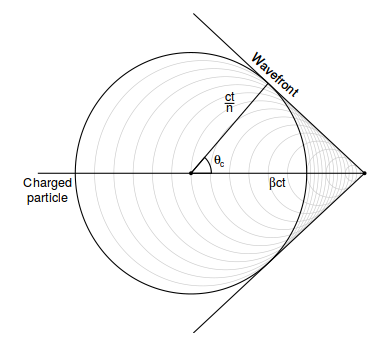
\includegraphics[width = 0.4\linewidth]{GeometriaCherenkov.png}
 
 Extra\'ido de \citep{BALDINI}
\caption{Geometr\'ia relevante en la radiaci\'on Cherenkov}
\end{center}
\end{figure}

\begin{equation}
\cos\theta_c=\frac{1}{\beta n}
\end{equation}

Notando aqu\'i que el \'indice de refracci\'on depende de la longitud de onda de la radiaci\'on. Para el agua, la radiaci\'on ocurre en el intervalo de longitudes de onda entre 300 y 570 nm. \citep{PEREZ}

Debido a que existe simetr\'ia en el \'angulo azimutal, la forma del frente de onda es un cono. Usando el caso cr\'itico cuando en la ecuaci\'on 5.2 $\cos\theta=1$, se puede obtener una expersi\'on para la energ\'ia m\'inima de una part\'icula para producir radiaci\'on Cherenkov.

\begin{equation}
E_c=\gamma m_0=\frac{m_o}{\sqrt{1-n^{-2}}}
\end{equation}

Para el agua, con $n=1.33$, toma un valor aproximado de $E_c\approx1.52m_0$. \citep{PEREZ}

El espectro (doble diferencial) de los fotones producidos por unidad de longitud $x$ y de longitud de onda $\lambda$ lo describe

\begin{equation}
\frac{d^2N}{dxd\lambda}=\frac{2\pi\alpha z^2}{\lambda^2}\Bigg(1-\frac{1}{\beta^2n^2(\lambda)}\Bigg)
\end{equation}

donde $z$ es la carga de la part\'icula y $\alpha$ es la constante de estructura fina. \citep{BALDINI}

La radiaci\'on de Cherenkov no es importante en t\'erminos de la energ\'ia perdida. En cambio, la existencia de un umbral de generaci\'on de radiaci\'on y la dependencia del \'angulo $\theta$ y del espectro sobre la velocidad de la part\'icula hacen la detetecci\'on de radiaci\'on Cherenkov \'util para la identificaci\'on de part\'iculas (evidenciado en la ecuaci\'on 5.3) y medici\'on de velocidades. \citep{BALDINI}

En el contexto de los detectores de rayos c\'osmicas terrestres en agua, las propiedades de la radiaci\'on de Cherenkov importantes son: la existencia del umbral dado por la ecuaci\'on 5.1; la cantidad de fotones emitidos por unidad de longitud tiende r\'apidamente a una constante que depende de $\lambda$, $n$ y la longitud recorrida. Es decir que la se\~nal del detector se relaciona con la cantidad de fotones producidos, y no con la energ\'ia depositada. De hecho, muy poco porcentaje de la energ\'ia depositada en un detector de agua es por radiaci\'on de Cherenkov; alrededor del 1 \% en gases de n\'umero at\'omico mayor a 7. En lugar, la mayor parte de la energ\'ia se pierde a trav\'es de otras interacciones de ionizaci\'on y excitaci\'on. \citep{PEREZ} \citep{GROUPENS}

Para obtener el n\'umero total de fotones emitidos en un contador de Cherenkov, se integra la ecuaci\'on 5.4 sobre toda la regi\'on en la cual se cumple $\beta n(\lambda) > 1$, y se convoluciona con la funci\'on de respuesta del sistema de recolecci\'on de luz. En el caso de los detectores de rayos c\'osmicos por radiaci\'on Cherenkov en agua (WCD por sus siglas en ingl\'es, de ahora en adelante), el sistema de recolecci\'on de luz es un tanque de agua purificada con paredes hechas de material altamente reflector.

\section{Latin American Giant Observatory}
\subsection{Sitios de LAGO}
LAGO (Latin American Giant Observatory, por sus siglas en ingl\'es) es un proyecto internacional con m\'as de ochenta cient\'ificos de ocho pa\'ises latinoamericanos que empez\'o en 2005. Est\'a orientado principalmente a la investigaci\'on b\'asica de tres ramas de la astrof\'isica de part\'iculas: el universo en condiciones extremas, clima interplanetario y radiaci\'on atmosf\'erica a nivel del suelo. La red de detectores de LAGO consiste en peque\~nos tanques de agua a nivel de tierra sobre diferentes localidades y latitudes a lo largo del continente latinoamericano, abarcando desde M\'exico hasta el cono sur de Am\'erica. El proyecto LAGO se ha dividi\'o en dos estudios objetivos dependiendo de la altitud del detector. Los detectores en altitudes superiores de 4,500m sobre el nivel del mar permiten detectar GRB con mayor sensibilidad; y los detectores de altitudes menores son utilizados para estudios f\'isicos del Sol (decrecimientos Forbush). \citep{ASOREY2015}

\begin{figure}[ht] %opci\'on h - here pone la imagen aqu\'i en esta posici\'on del documento
\begin{center}
 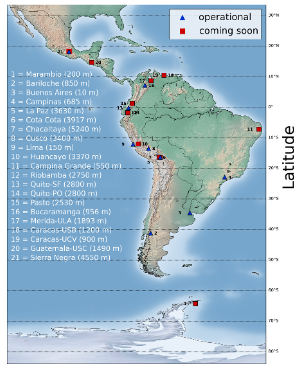
\includegraphics[width = 0.5\linewidth]{ASOREY2015.png}
 
 Extra\'ido de \citep{ASOREY2015}
\caption{Distribuci\'on geogr\'afica de los detectores de LAGO operacionales (tri\'angulos), y los que comenzar\'an a funcionar entre 2016 y 2017 (cuadrados)}
\end{center}
\end{figure}

LAGO tiene como objetivo observar Gamma Ray Bursts (GRB) (destellos de rayos gamma) utilizando WCD. Los detectores de LAGO pueden ser utilizados para medir el flujo de rayos c\'osmicos en la tierra ya que su modulaci\'on es una medici\'on directa de la actividad solar. Por \'ultimo, los detectores instalados en universidades sirven para ense\~nar a estudiantes sobre f\'isica de part\'iculas y astropart\'iculas. Existen ya varios observatorios de LAGO en operaci\'on. Uno de ellos est\'a en Sierra Negra, M\'exico, a 4550 metros sobre el nivel del mar. Tiene funcionando tres tanques de 4 metros cuadrados de superficie y dos de un metro cuadrado. Otro est\'a en Chacaltaya, Bolivia, a 5250 metros sobre el nivel del mar, el detector a mayor altitud de la estructura LAGO. Tiene tres tanques en operaci\'on, dos de 4 metros cuadrado y uno de 1 metro cuadrado. El otro est\'a en Marcapomacocha, Per\'u, a 4450 metros sobre el nivel del mar, con un tanque de dos metros cuadrados en operaci\'on desde el 2010. En Guatemala, ya dio inicio el proyecto en la Universidad San Carlos de Guatemala, pero a\'un no est\'a en operaci\'on. \citep{VILLASENOR}

\subsection{Detectores Cherenkov de LAGO}

La base de los detectores en LAGO es un tanque cil\'indrico de material como resina de polietileno. Est\'a recubierto en el exterior por una capa de material que evita el ingreso de luz externa, como manto asf\'altico o pl\'astico de polietileno negro. La superficie interior est\'a recubierta por una manta de Tyvek, que es un material altamente reflectivo. La superficie del Tyvek consiste en fibras de polietileno de alta densidad de 5-10 $\mu$m orientadas de forma aleatoria y no direccional. Dentro, se llena con agua purificada. \citep{PEREZ} \citep{DUPONT}

\begin{figure}[ht] %opci\'on h - here pone la imagen aqu\'i en esta posici\'on del documento
\begin{center}
 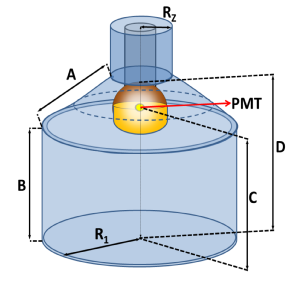
\includegraphics[width = 0.5\linewidth]{DetectorLAGO.png}
 
 Extra\'ido de \citep{PEREZ}
\caption{Diagrama de un detector t\'ipico de la colaboraci\'on LAGO}
\end{center}
\end{figure}

Algunas ventajas del Tyvek es que no se degrada en mayor manera en contacto con agua y tiene buena resistencia mec\'anica, pero su propiedad m\'as importante es que tiene una reflectividad en aire en el espectro visible del 90\%, y disminuye a 86\% a 360nm y al 78\% a 320nm; rangos en los que se encuentra la longitud de onda de emisi\'on de radiaci\'on Vavilov-Cherenkov y la sensibilidad normal del fotomultiplicador (PMT, por sus siglas en ingl\'es, de ahora en adelante). Generalmente se coloca el PMT en la tapa superior del tanque. El agua entra en contacto \'unicamente con el Tyvek y con el vidrio de detecci\'on del fotomultiplicador. \citep{PEREZ}

El agua, junto al Tyvek y el fotomultiplicador, constituyen el sistema de recolecci\'on de fotones de la radiaci\'on Cherenkov que ocurre en el agua. Estos fotones son reflejados en las paredes del Tyvek hasta alcanzar el fotomultiplicador. De hecho, un bajo porcentaje de fotones logra alcanzar el fotomultiplicador. Este porcentaje se aproxima como el cociente del \'area de detecci\'on y el \'area superficial interna del tanque. La cantidad de fotones detectados son suficientes para generar una se\~nal distinguible en el detector. El constante mantenimiento de la calidad del agua facilita la calibraci\'on de los tanques, ya que se ha observado que la degradaci\'on de la calidad de agua disminuye la capacidad del sistema de recolecci\'on de fotones. \citep{PEREZ}

\subsection{Tubo fotomultiplicador}

Los tubos fotomultiplicadores son detectores al vac\'io extremadamente sensibles a luz en el rango visible, ultravioleta e infrarrojo. Logran amplificar la corriente producida por luz incidente hasta 100 millones de veces, por lo que son capaces de detectar pocos fotones incidentes. Consisten en una ventana de ingreso (un vidrio de borosilicato, por ejemplo), un fotoc\'atodo, un electrodo para enfocar, un multiplicador de electrones (d\'inodos en secuencia) y un \'anodo, todo sellado en un tubo de vidrio al vac\'io. El diagrama en la figura 5.5 muestra la construcci\'on b\'asica de un PMT. \citep{Hamamatsu}

\begin{figure}[ht] %opci\'on h - here pone la imagen aqu\'i en esta posici\'on del documento
\begin{center}
 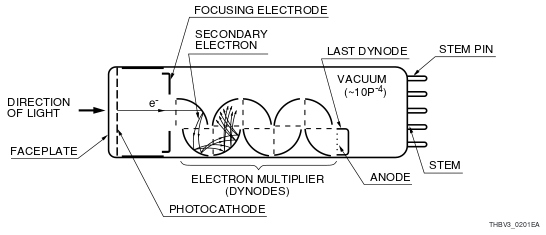
\includegraphics[width =0.8\linewidth]{Hamamatsu.png}
 
 Extra\'ido de \citep{Hamamatsu}
\caption{Construcci\'on b\'asica de un PMT}
\end{center}
\end{figure}

Primero, la  luz ingresa por la ventana de vidrio. Al chocar con el fotoc\'atodo, los fotones excitan y desprenden fotoelectrones por efecto fotoel\'ectrico hacia el vac\'io del tubo. El electrodo acelera y dirige esta corriente hacia los d\'inodos. Estos constituyen el multiplicador de electrones: entre los d\'inodos se coloca un alto voltaje, que provoca que los electrones incidentes sean multiplicados por efecto de emisi\'on secundaria de electrones. \citep{Hamamatsu}

El multiplicador de electrones es el responsable de producir la dram\'atica amplificaci\'on de corriente, porque cada d\'inodo contribuye a una cascada multiplicativa de electrones: para un fototubo de $N_d$ d\'inodos, la corriente final habr\'a tenido una ganancia de $\delta^{N_d}$, con $\delta$ siendo t\'ipicamente alrededor de 6-7 electrones. En LAGO, se usan fototubos con un \'area de detecci\'on de alrededor de 9 pulgadas y multiplicadores de electrones de 10-12 d\'inodos. El \'anodo es un electrodo que recolecta los electrones secundarios multiplicados en el proceso de cascada y arroja la corriente a un circuito externo. Lo m\'as importante en el dise\~no del \'anodo es una diferencia de potencia adecuada entre el \'ultimo d\'inodo y el \'anodo para obtener la mayor corriente de salida. \citep{Hamamatsu}

\begin{figure}[ht] %opci\'on h - here pone la imagen aqu\'i en esta posici\'on del documento
\begin{center}
 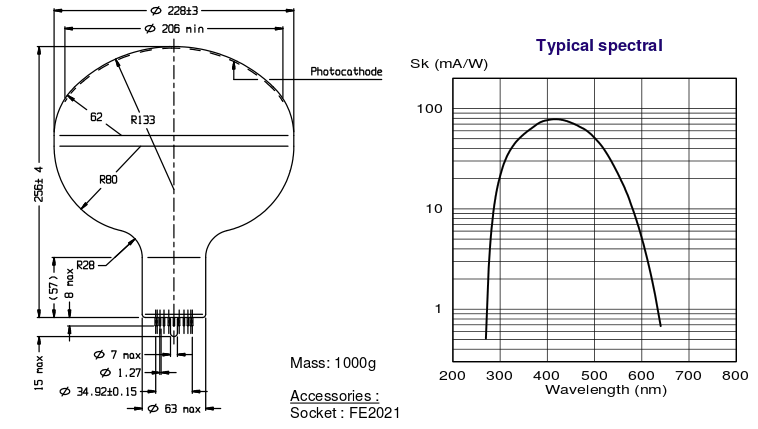
\includegraphics[width =0.8\linewidth]{PhotonisXP1802.png}
 
 Extra\'ido de \citep{Photonis}
\caption{Diagramas de a) la construcci\'on b\'asica de Photonis XP1802 con dimensiones dadas en mm y b) su espectro de radiaci\'on}
\end{center}
\end{figure}

Una propiedad importante de un PMT es su eficiencia cu\'antica o su espectro de radiaci\'on. Ambos miden la eficiencia del PMT de convertir la energ\'ia de los fotones en corriente. La eficiencia cu\'antica mide el cociente entre la cantidad de fotoelectrones emitidos por el fotoc\'atodo y el n\'umero de fotones incidentes, expresado en porcentaje. El espectro de radiaci\'on mide la corriente de electrones producido por el fotoc\'atodo dividido el flujo de radiaci\'on para alguna longitud de onda, y se mide en amperios por vatio. La conversi\'on entre eficiencia cu\'antica ($QE_\lambda$) y espectro de radiaci\'on ($R_\lambda$) es

\begin{equation}
QE_\lambda=R_\lambda\frac{E_\lambda}{e}=\frac{R_\lambda}{\lambda}\frac{hc}{e}
\end{equation}

donde $\lambda$ es la longitud de onda de la luz incidente, $E_\lambda=\frac{hc}{\lambda}$ es la energ\'ia del fot\'on incidente, $e$ es la carga elemental, $c$ es la velocidad de la luz en el vac\'io y $h$ es la constante de Planck.

Por el efecto fotoel\'ectrico, la probabilidad de emisi\'on aumenta para longitudes de onda m\'as bajas (ya que estos fotones poseen m\'as energ\'ia). Por esto, la eficiencia cu\'antica est\'a dada respecto a la longitud de onda de los fotones incidentes. En este megaproyecto se utiliz\'o un PMT marca Photonis XP1802, cuyo espectro de radiaci\'on y construcci\'on b\'asica est\'an dados en la figura 5.6. La eficiencia cu\'antica de este PMT es de 23 \% a una longitud de onda de 420nm. \citep{Hamamatsu} \citep{Photonis}

\subsection{Electr\'onica de LAGO}
La se\~nal an\'aloga del PMT es digitalizada por conversores anal\'ogico-digital (FADC por sus siglas en ingl\'es) de 10 a 14 bits a una velocidad de muesstro de 40MHz. Esta velocidad de muestreo define la resoluci\'on de la electr\'onica por

\begin{equation}
1 bin\equiv\frac{1}{40MHz}=25ns
\end{equation}

Con el FADC, la se\~nal en voltaje se convierte en una medici\'on de cuentas digitales, $ADC$. El valor de $ADC$ pico, $ADC_p$ corresponde al valor de salida del FADC, en un rango de 0 a $2^10-1=1024$ cuentas. El rango de entrada para esto es entre 0 a 2 V. A partir de esto, se tiene la equivalencia

\begin{equation}
1 ADC_p\equiv\frac{2V}{2^{10}}=1.95mV
\end{equation}

La digitalizaci\'on ocurre en la placa digitalizadora, que puede procesar se\~nales simult\'aneamente en tres canales y utiliza conversores AD9203 marca Analog Devices. La se\~nal digitalizada es tratada por la Nexys-2, de la empresa Digilent, que es un kit al que se pueden montar sensores como el sensor HP03S que miden la presi\'on absoluta y temperatura y sistema GPS. \citep{ARNALDI} \citep{PEREZ}

\begin{figure}[h] %opci\'on h - here pone la imagen aqu\'i en esta posici\'on del documento
\begin{center}
 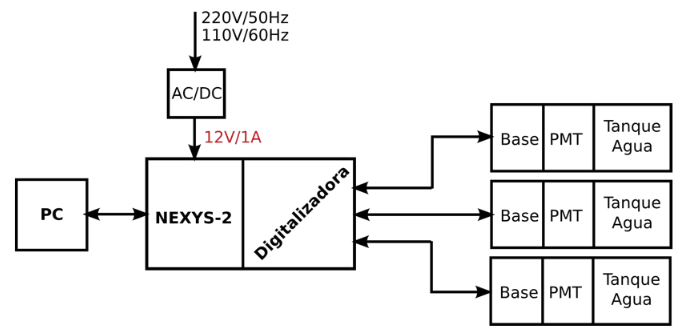
\includegraphics[width =0.8\linewidth]{ElectronicaLAGO.png}
 
 Extra\'ido de \citep{SOFO}
\caption{Diagrama de bloques de la electr\'onica LAGO para tres tanques, mostrando el kit de desarrollo Nexys 2 conectada a una fuente externa y la targeta digitalizadora}
\end{center}
\end{figure}

\subsection{ACQUA y ANNA de LAGO}
ACQUA es un sistema de adquisici\'on de datos  desarrollado para el proyecto LAGO que tiene como objetivo estandarizar el formato de los datos y su an\'alisis adquiridos por las diferentes estaciones. Cada estaci\'on del proyecto LAGO puede utilizar este c\'odigo adem\'as para subir sus datos al repositorio central. El c\'odigo sirve para operar la electr\'onica, identific\'ando los datos adquiridos con las caracter\'isticas importantes de la estaci\'on. Estas incluyen la posici\'on geogr\'afica, altitud, instituci\'on, modelo de PMT, n\'umero de detectores, geometr\'ia del detector y otras especificaciones de electr\'onica.

\begin{figure}[h] %opci\'on h - here pone la imagen aqu\'i en esta posici\'on del documento
\begin{center}
 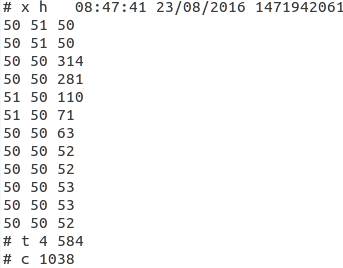
\includegraphics[width =0.5\linewidth]{PulsoADC.png}
 
(Fuente propia)
\caption{Formato de un pulso en el archivo crudo producido con el sistema de adquisici\'on ACQUA}
\end{center}
\end{figure}

La figura 5.8 muestra el formato de los pulsos en los datos crudos. El primer pulso en la figura es el primero de la adquisici\'on. La l\'inea al inicio da el tiempo en que comenz\'o el proceso, lo toma del GPS o, en ausencia del GPS, del tiempo de la computadora. Un pulso se almacena cuando la se\~nal supera un umbral dado. Las filas siguientes de tres columnas muestran la cuenta en ADC para cada canal, en la configuraci\'on mostrada, se us\'o \'unicamente el canal 3, con una l\'inea base de 50 ADC. Las \'ultimas dos l\'inea del pulso tienen informaci\'on del tiempo en que se almacen\'o el pulso (en unidades de $bin$, como dado en la ecuaci\'on 5.5) y el identificador interno de pulso (un contador).

ANNA es la \textit{suite} de an\'alisis de datos oficial de LAGO. El c\'odigo principal es "raw.cc", que convierte los datos crudos adquiridos por el c\'odigo de ACQUA al primer nivel de datos pre-analizados. Los resultados del c\'odigo pueden ser archivos con la carga integrada temporalmente de los pulsos, archivos de histogramas de la diferencia de tiempos, archivos con el conteo total por segundo, entre otros. La documentaci\'on entera de ACQUA y ANNA se puede encontrar en la wiki oficial de LAGO, en wiki.lagoproject.org.

\section{Identificaci\'on de part\'iculas en detectores de Cherenkov terrestres}

\subsection{Relaci\'on entre tiempo de subida y amplitud}

En \citep{Salazar}, se desarroll\'o un procedimiento experimental para identificar muones verticales y muones arbitrarios. Los muones verticales se seleccionan cuando coinciden dos hodoscopios colocados como en la figura 5.9, y muones arbitrarios se escogen cuando la se\~nal superaba un umbral de de 30mV.

\begin{figure}[h] %opci\'on h - here pone la imagen aqu\'i en esta posici\'on del documento
\begin{center}
 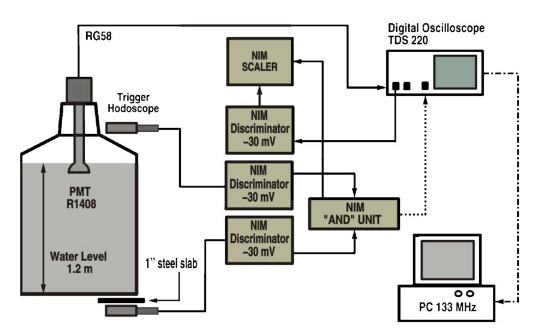
\includegraphics[width =0.8\linewidth]{WCDSalazar.png}
 
 Extra\'ido de \citep{Salazar}
\caption{Diagrama esquem\'atico del WCD y del sistema de adquisici\'on usado en \citep{Salazar}, mostrando el uso de hodoscopio para la identificaci\'on de muones verticales}
\end{center}
\end{figure}

Los hodoscopios tienen una pieza centelladora que produce luz y se\~nal (a trav\'es de un diodo o un PMT) cuando una part\'icula cargada lo atraviesa. Eventos identificados como producidos por electrones eran en su mayor medida generados por el decaimiento de muones al chocar con paredes de concreto en el laboratorio. Los electrones producidos en el decaimiento de muones siguen una distribuci\'on de Michael, con un valor promedio de energ\'ia de 37 MeV. \citep{ALLISON}

La importancia de esta clasificaci\'on es que se gener\'o la gr\'afica mostrada en la figura 5.9, que muestra la relaci\'on entre tiempo de subida y amplitud para los diferentes fuentes de pulso. Para validar esta interpretaci\'on, graficaron los eventos que aparecen cuando el hodoscopio se alinea con el vidrio del PMT. La propiedad m\'as importante a destacar en esta gr\'afica son las posiciones generales de los eventos de electrones comparadas con las de muones: los eventos de electrones generados por decaimiento tienen tiempos de subida menores y amplitudes iguales o mayores que los de muones. \citep{Salazar}

\begin{figure}[h] %opci\'on h - here pone la imagen aqu\'i en esta posici\'on del documento
\begin{center}
 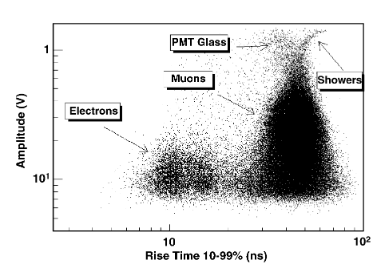
\includegraphics[width =0.8\linewidth]{RiseTimeAmpSalazar.png}
 
 Extra\'ido de \citep{Salazar}
\caption{Amplitud respecto al tiempo de subida 10 a 90\% para la clasificaci\'on de muones arbitrarios}
\end{center}
\end{figure}

\subsection{Modo Histograma en LAGO}
Las part\'iculas secundarias que entran al tanque producen radiaci\'on de Cherenkov en su recorrido que finalmente se detecta como pulsos medidos en unidades ADC. Una medida de la cantidad de fotones de radiaci\'on Cherenkov detectados es la carga integrada ADCq. Esta se calcula tomando el pulso medido en ADCq, restando el valor de la l\'inea base, e integrando temporalmente. Un histograma de los eventos ADCq revela cierta estructura del tipo de part\'iculas que ingresan al tanque y una manera independiente de identificarlas. \citep{PEREZ}

\begin{figure}[ht] %opci\'on h - here pone la imagen aqu\'i en esta posici\'on del documento
\begin{center}
 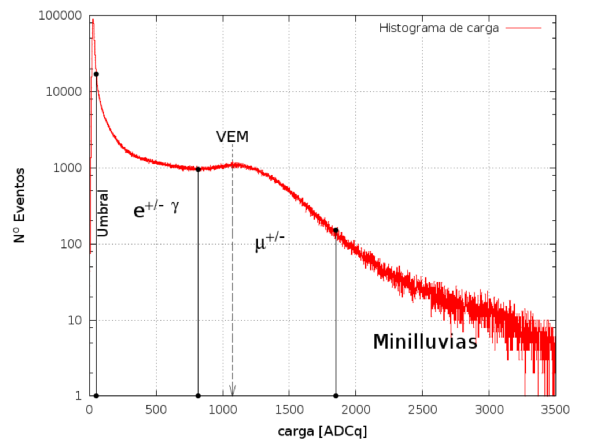
\includegraphics[width =0.8\linewidth]{HistogramaNahuelito.png}
 
 Extra\'ido de \citep{PEREZ}
\caption{Histograma de carga integrada en ADCq (en el eje horizontal) t\'ipico para un WCD, tomado con datos de Nahuelito}
\end{center}
\end{figure}

La propiedad m\'as importante de histogramas de carga integrada en ADCq es la presencia de un segundo m\'aximo, por sobre la acumulaci\'on de se\~nales que podr\'ian interpretarse como ruido. Esto se muestra en la figura 5.10, obtenida de datos de Nahuelito en \citep{PEREZ}. La ubicaci\'on de este m\'aximo corresponde a pulsos generados por el paso de muones verticales. Este valor en ADCq es utilizado para calibrar el detector. El modo histograma presentado en \citep{PEREZ} establece un procedimiento para clasificar eventos a partir de puntos cr\'iticos del histograma de ADCq.

Los tres valores cr\'iticos que utiliza son el primer m\'aximo $em_{peak}$, el primer m\'inimo (llamado punto de transici\'on) y el VEM antes mencionado. El VEM adem\'as define un punto de ADCq mayor, dado por muones que atraviesan el detector en su diagonal. Este valor $mu_{max}$ se calcula mediante

\begin{equation}
mu_{max}=0.9\times VEM\times\sqrt{1+\Bigg(\frac{d}{h}\Bigg)^2}
\end{equation}

donde $d$ es el di\'ametro del tanque, $h$ es su altura y el factor 0.9 es para tomar en cuenta la contaminaci\'on por eventos no mu\'onicos.

Estos dividen los eventos en tres bandas: la banda electromagn\'etica para eventos con carga integrada menor al del punto de transici\'on, la de componente mu\'onica entre el punto de transici\'on y $mu_{max}$, y de minilluvias para los de mayor ADCq. La banda electromagn\'etica corresponde a electrones, positrones y fotones de alta energ\'ia que por interacci\'on producen electrones y positrones. La componente mu\'onica son los muones provenientes de cascadas de \'area extensa que atraviesan el tanque por la tapa superior. La banda de minilluvias son part\'iculas secundarias de las cascadas de \'area extensa cuya diferencia temporal es mayor a la resoluci\'on del detector. \citep{PEREZ}

La clasificaci\'on de part\'iculas por el modo histograma permite un an\'alis m\'as detallado de la modulaci\'on solar sobre el conteo de rayos c\'osmicos. Esto se logra estudiando la evoluci\'on temporal del conteo de eventos por clasificaci\'on para encontrar decrecimientos Forbush. La diferencia entre las evoluciones temporales relativas de cada banda de eventos revela interacciones de las eyecciones de masa coronal interplanetarias con la magnet\'osfera terrestre. \citep{PEREZ}

\section{Simulaci\'on Geant4 de detectores Cherenkov en agua}

Para realizar las simulaciones de GEANT4 se siguieron las gu\'ias de desarrollador de aplicaci\'on y se tomaron de referencias otros art\'iculos con simulaciones parecidas, \citep{NIELSEN}, \citep{CHEN}, \citep{CALDERON}.

\subsection{Modelos f\'isicos y fotones \'opticos}
Los fotones \'opticos (\textit{opticalphotons}) en la simulaci\'on Geant4 son fotones con longitudes de onda mucho mayores que el espacio t\'ipico entre \'atomos, o sea, $\lambda\geq 10nm$. La producci\'on de fotones \'opticos se debe principalmente al efecto Cherenkov y procesos de centellos. Las tres interacciones para fotones \'opticos son la dispersi\'on el\'astica (Rayleigh), absorci\'on e interacciones en superficies. La primera usualmente no es importante, ya que la distancia de camino medio es alrededor de 1.7 km para longitudes de onda de radio. La absorci\'on, en cambio, s\'i es importante, ya que determina el l\'imite inferior de longitud de onda para la transparencia del material. La \'ultima interacci\'on se describe en la siguiente secci\'on.

La simulaci\'on trabaja el efecto Cherenkov primero calculando el n\'umero de fotones por unidad de longitud, dada por la ecuaci\'on 5.4, y de acuerdo al umbral de velocidad y el \'angulo en la ecuaci\'on 5.2 genera fotones \'opticos por cada paso de la simulaci\'on.

\subsection{Efectos en los bordes de volumen}
El comportamiento de un fot\'on cuando arriba al borde de un material depende de la naturaleza de los dos materiales que se unen en el borde. El primer caso es dos materiales diel\'ectricos, en el que el fot\'on puede ser transmitido o reflejado. El segundo es cuando pasa de un material diel\'ectrico a uno que se comporta como metal, entonces puede ser absorbido (y detectado, seg\'un la superficie) o reflejado. El tercer caso es cuando arriba a un material para el cual no se ha especificado ninguna propiedad \'optica, en ese caso el fot\'on es absorbido.

Los modelos \textit{UNIFIED} y \textit{GLISUR} son modelos que integran las principales caracter\'isticas de modelos \'opticos geom\'etricos y f\'isicos para reflexi\'on y transmisi\'on en superficies en diferentes longitudes de onda y aspereza. La diferencia entre los modelos est\'a en c\'omo dan la distribuci\'on de la direcci\'on de la reflexi\'on de fotones.

\begin{itemize}
\item \textit{UNIFIED} modela esta distribuci\'on como proporcional a la gaussiana de un par\'ametro de aspereza (llamado \textit{sigma\_alpha} y medido en radianes).
\item \textit{GLISUR}	toma un par\'ametro de aspereza diferente \textit{polish}, que toma valores de 0 (m\'axima aspereza) a 1 (m\'inima aspereza), crea una esfera con radio \textit{polish}, escoge un punto al azar en su superficie y agrega el vector de la normal en ese punto a la direcci\'on de reflexi\'on.
\end{itemize}

\begin{figure}[h] %opci\'on h - here pone la imagen aqu\'i en esta posici\'on del documento
\begin{center}
 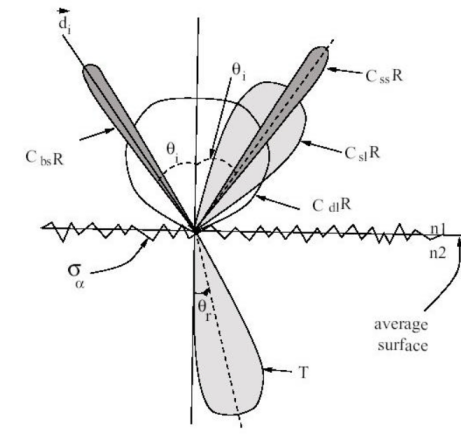
\includegraphics[width = 0.5\linewidth]{UNIFIED.png}
 
 $C_bsR$: Reflexi\'on por retrodispersi\'on\\
 $C_dlR$: Reflexi\'on Lambertiana interna\\
 $C_ssR$: Reflexi\'on con la normal de la superficie promedio\\
 $C_slR$: Reflexi\'on con la normal de la rugosidad\\
 $\theta_i$: \'Angulo de incidencia\\
 $T$: Transmisi\'on\\
 $\theta_r$: \'Angulo de transmisi\'on\\
 $\sigma_\alpha$: Aspereza\\
 Extra\'ido y modificado de \citep{GUMP}
\caption{Ilustriaci\'on de las posibles reflexiones que el modelo \textit{UNIFIED} calcula para la direcci\'on de reflexi\'on de fotones \'opticos incidentes a superficies \'asperas. Las \'areas sombreadas ilustran la probabilidad gaussiana de cada reflexi\'on.}
\end{center}
\end{figure}

Geant4 incluye la radiaci\'on Cherenkov como un proceso f\'isico que puede implementarse desde los archivos de procesos f\'isicos. Calcula las secciones eficaces a partir de la descripci\'on molecular del material refractor. 

%%%%%%%%%%%%%%%%Cap\'itulo nuevo

\Chapter{Metodolog\'ia}

\section{Simulaci\'on}
El objetivo del experimento fue caracterizar las se\~nales de part\'iculas que inciden en el tanque. Para la simulaci\'on, se decidi\'o analizar los pulsos de muones de alrededor de 4 GeV de energ\'ia, rayos gamma de 100 MeV de energ\'ia y electrones de 37 MeV de energ\'ia. Los primeros son muones provenientes de la cascada mu\'onica, que por su alta energ\'ia no decaen dentro del tanque. Los rayos gamma son part\'iculas que se obtendr\'ian con mayor frecuencia en el tanque a mayores altitudes, por lo que servir\'a para futuros proyectos. Los electrones de 37 MeV son electrones con la energ\'ia promedio de la distribuci\'on de Michael, producidos por el decaimiento de muones dentro del tanque. Estos electrones depositan toda su energ\'ia dentro del tanque y seg\'un \citep{ALLISON} sirven para calibrar el instrumento debido a que su energ\'ia ocurre en el primer pico en los histogramas de carga del experimento.

Para la simulaci\'on se utiliz\'o el programa Geant4, desarrollado por CERN para simulaci\'on de experimentos de part\'iculas. El paquete de descarga incluye ejemplos b\'asicos y avanzados de experimentos que se utilizaron de referencia para el desarrollo del presente. En particular, mucho del c\'odigo se bas\'o en los ejemplos OpNovice (que implementa la radiaci\'on Cherenkov) y HitLXE (que utiliza fotomultiplicadores). El desarrollo del programa fue auxiliado por el trabajo de H\'ector P\'erez durante todo el proceso; ambos programas est\'an disponibles en el repositorio https://github.com/hepfpeh/Geant4-WCD.git.
\subsection{Geometr\'ia}
\subsubsection{Objetos y colocaci\'on}

Los objetos de la construcci\'on del detector relevantes para la simulaci\'on son los objetos con los que interact\'uan los fot\'ones \'opticos y los secundarios incidentes dentro del tanque. Estos objetos son el recubrimiento de Tyvek, que se toma como un capa cil\'indrica, el agua dentro del Tyvek, la superficie de vidrio borosilicato del fotomultplicador y el fotoc\'atodo de aluminio, ambos tomados como semiesferas. Geant4 permite organizar objetos seg\'un jerarqu\'ias: el cuadro 10.1 en el cap\'itulo de Anexos describe la forma, dimensiones y colocaci\'on de los objetos y sus jerarqu\'ias bajo los respectivos vol\'umenes madre. Las dimensiones del Tyvek y de las semiesferas que conforman la parte del fotomultiplicador en contacto con el agua fueron medidas directamente del tanque del experimento. Esta geometr\'ia se expone visualmente en la figura 6.1.

\begin{figure}[h] %opci\'on h - here pone la imagen aqu\'i en esta posici\'on del documento
\begin{center}
 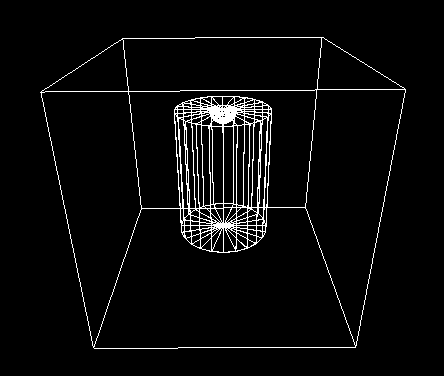
\includegraphics[width = 0.8\linewidth]{GeometriaG4.png}
 
(Fuente propia)
\caption{Ilustraci\'on de la geometr\'ia general del detector en la simulaci\'on Geant4, mostrando el recubrimiento Tyvek en forma cil\'indrica y las superficies de vidrio y fotoc\'atodo del fotomultiplicador}
\end{center}
\end{figure}

\subsubsection{Materiales}
Los materiales se tomaron del cat\'alogo de NIST de Geant4, y con la clase G4MaterialsPropertiesTable se asignaron valores de \'indices de refracci\'on y largo de atenuaci\'on al agua correspondientes a una lista de energ\'ia de fot\'on (para las tablas completas, ver el cuadro 10.2 en Anexos) y el \'indice de refracci\'on del borosilicato se tom\'o como 1.50. El vac\'io se model\'o como gas hidr\'ogeno a una temperatura de 0.1 kelvin y con la densidad promedio del universo.

\subsubsection{Superficies}
Se especificaron dos superficies: la superficie entre el agua y el recubrimiento de Tyvek, y el borde del fotoc\'atodo. Ambos bordes se crearon con la clase G4OpticalSurface, y son 
\begin{itemize}
\item Agua-Tyvek: El tyvek se coloc\'o como volumen madre del agua para que ambos estuvieran completamente en contacto en el borde del volumen del agua (a excepci\'on del contacto del agua con el vidrio de borosilicato). Esta superficie es de tipo diel\'ectrico-metal (reflexi\'on o absorci\'on), terminado \textit{ground} por la aspereza del Tyvek, y se le asign\'o el modelo \textit{unified} de Geant4. Los detalles de las propiedades que se especificaron para esta superficie se asignaron usando una tabla de propiedades de material (\textit{G4MaterialPropertiesTable}), que se resumen en el cuadro 6.1.
\item Fotoc\'atodo: El fotoc\'atodo es el volumen de detecci\'on de la simulaci\'on, por lo que en su superficie se especific\'o una eficiencia de 1 (la eficiencia cu\'antica se tom\'o en cuenta luego en forma de la respuesta espectral para la generaci\'on de pulsos). Se cre\'o de tipo diel\'ectrico-metal (reflexi\'on o absorci\'on), con terminado \textit{polished} y se le asign\'o el modelo \textit{glisur} de Geant4 (sin embargo, debido a que se tom\'o como superficie lisa, los efectos de superficie no son relevantes y el modelo no es usado)
\end{itemize}

\begin{table}[h]
\caption{ Descripci\'on de las propiedades de la superficie Agua-Tyvek asignadas para dos energ\'ias de fot\'on}
\centering
\begin{tabular}{l c c c c c }
\hline
\specialcell{Energ\'ia del\\fot\'on(eV)} & Reflectividad & Eficiencia & \specialcell{Coeficiente de\\refracci\'on} & \specialcell{Constante\\especular} & \specialcell{Constante\\retrodispersi\'on}  \\ \hline
2.034 & 0.2534 & 0 & 1.333 & 0.3 & 0.2 \\
4.136 & 0.2534 & 0 & 1.333 & 0.3 & 0.2 \\

\hline
\end{tabular}
\end{table}

Los valores de reflectividad del Tyvek y el \'indice de refracci\'on del agua fueron obtenidos por Karen Gu\'arcax para este megaproyecto en el m\'odulo de "Medio de distribuci\'on de detector de radiaci\'on Vavilov-Cherenkov" mediante un experimento de reflectividad del Tyvek sumergido en jarras con agua y con la refracci\'on en agua de la luz de una l\'ampara de sodio.

\subsection{Detecci\'on}
Se defini\'o al fotoc\'atodo como detector asign\'andolo como el \textit{SensitiveDetector}. Con la clase \textit{ProcessHits} se registr\'o cada vez que un fot\'on entra en contacto con el fotoc\'atodo y se guard\'o el tiempo de detecci\'on de cada fot\'on y el conteo total.

\subsection{Generaci\'on de evento}

\subsubsection{Procesos f\'isicos}
Se utiliz\'o el modelo de fotones \'opticos. Los procesos f\'isicos y las clases respectivas se incluyeron en el archivo "KinichAhauPhysicsList".

\subsubsection{Posici\'on y direcci\'on}
La simulaci\'on consisti\'o en dos partes, una para obtener los pulsos caracter\'isticos de cada tipo de part\'icula incidente y otra parte para obtener la cantidad de fotones detectados; esta \'ultima es proporcional a la medida de carga integrada (ADCq) del WCD. Para la primera se definieron la posici\'on y direcci\'on de las part\'iculas incidentes como constantes de tal manera que atravesaran el tanque completo verticalmente.

En la segunda parte del experimento se utiliz\'o una distribuci\'on uniforme sobre la tapa superior del tanque para definir la posici\'on, una distribuci\'on uniforme para el \'angulo azimutal (medido paralelo a la horizontal), y una distribuci\'on dada por $cos^2(\theta)$ para el \'angulo polar (medido respecto a la vertical). Para definir $\theta$, se utiliz\'o muestreo por rechazo para obtener valores de theta seg\'un la distribuci\'on.

\begin{figure}[h] %opci\'on h - here pone la imagen aqu\'i en esta posici\'on del documento
\begin{center}
 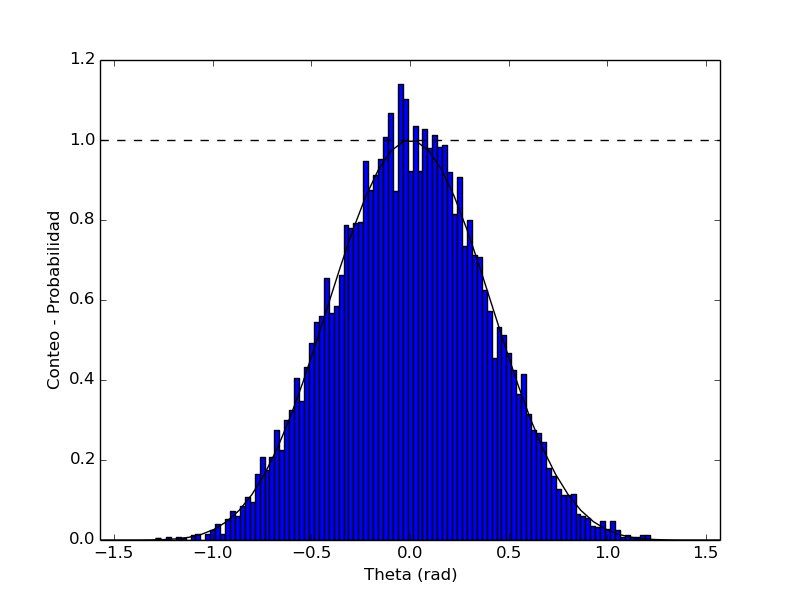
\includegraphics[width=\linewidth]{ThetaDist.png}

(Fuente propia)
\caption{Distribuci\'on para el \'angulo $\theta$ generadas por el algoritmo del muestreo por rechazo (histograma) y la curva $\cos^2(\theta)$}
\end{center}
\end{figure}

\subsection{Datos de salida}

Los tres tipos de salida principales fueron el n\'umero total de fotones producidos por evento, el n\'umero total de fotones detectados por evento, y el tiempo de cada detecci\'on. La cantidad de fotones producida se obtuvo con el archivo "KinichAhauStackingAction" verificando la producci\'on de fotones \'opticos secundarios en cada paso del \textit{track}. El n\'umero total de fotones detectados y su tiempo de detecci\'on se obtuvo imprimiendo el valor de \textit{GetGlobalTime()} del \textit{track} cada vez que un fot\'on \'optico entra en contacto con el fotoc\'atodo y agregando un contador. Todos estos datos se imprim\'ian por \textit{event}; usando el modo \textit{batch} de Geant4 desde la terminal, se guardaron directamente a un archivo ".txt".

Los primeros dos tipos de datos de salida se utilizaron para investigar c\'omo son sus distribuciones para eventos repetidos y para determinar si la energ\'ia de muones verticales incidentes est\'a correlacionada con la cantidad de fotones detectados. La literatura predice que la se\~nal obtenida del fototubo para muones verticales que atraviesan depende principalmente de la longitud del tanque.

El tercer tipo de salida se utiliz\'o para la caracterizaci\'on de los pulsos generados por a) muones verticales que atraviesan (4GeV), b) part\'icula gamma de 100 MeV (detectable a grandes altitudes) y c) electrones de Michael producidos por el decaimiento de muones en el tanque (37 MeV). Cada fot\'on excita una cantidad de electrones en el fotoc\'atodo, produciendo coriente en el fotomultiplicador. Esta corriente est\'a dada por la respuesta espectral del PMT, que para la longitud de onda de inter\'es es de 80 mA/W para una longitud de onda de 405 nm. Cada detecci\'on carga al multiplicador y la corriente producida decae como en un circuito RC.

\begin{equation}
I(t)=I_0e^{t/\tau}
\end{equation}

Donde $Tau$ se determin\'o experimentalmente alimentando el osciloscopio directamente del fotomultiplicador, arrojando un valor $18.76\pm0.03$. Se desarroll\'o un programa para generar pulsos del PMT a partir de los tiempos de detecci\'on (el programa est\'a completo en la secci\'on de Anexos). Se calcularon los intervalos de confianza (95\%) del valor de amplitud para cada tiempo de todos los pulsos respectivos para cada tipo de part\'icula y as\'i obtener los pulsos caracter\'isticos. Tambi\'en se realizaron gr\'aficas de amplitud (valor m\'aximo del pulso) versus tiempo de subida (tiempo en nanosegundos en que toma la se\~nal desde 0\% a 100\%) para cada tipo de evento, para investigar diferencias visibles en las gr\'aficas de cada uno y compararlo con lo encontrado en \citep{Salazar}

\section{Instalaci\'on del WCD "Kinich Ahau"}
Se bautiz\'o al tanque como Kinich Ahau. Se utiliz\'o como base del detector un tanque bicapa de polietileno de 600L marca Talishte. Se limpi\'o y procedi\'o a colocar el Tyvek en el interior, sujetado con una estructura de PVC. Se ajust\'o la estructura de tal manera que la distribuci\'on del difusor fuera uniforme dentro del tanque. Se enjuag\'o con agua municipal, para remover posibles contaminantes en la parte interna del tanque. Se recubri\'o la parte externa del tanque con vinilo de fibra de carbono DI-NOC marca 3M, para eliminar cualquier posible entrada de radiaci\'on electromagn\'etica que se encuentre en el rango de detecci\'on del PMT (300nm a 650nm). Para las primeras corridas durante agosto del 2016, se utiliz\'o agua municipal.

\begin{figure}[h] %opci\'on h - here pone la imagen aqu\'i en esta posici\'on del documento
\begin{center}
 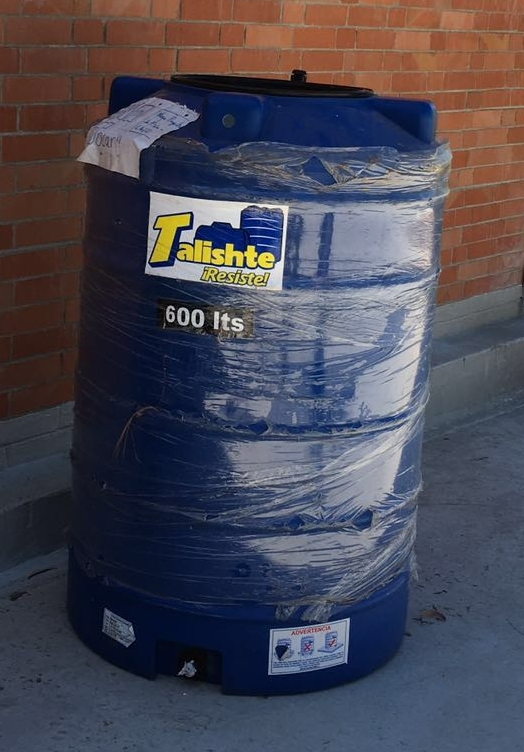
\includegraphics[width = 0.35\linewidth]{Talishte.jpg}

(Fuente propia)
\caption{Tanque de polietileno, de 600L marca Talishte utilizado como base del detector}
\end{center}
\end{figure}

Luego se instal\'o la electr\'onica seg\'un la gu\'ia oficial de electr\'onica de LAGO, elaborada (\textit{LAGO Official Electronics guide}) por M. Sofo, H. Arnaldi, G. Asorey y M. Gomez. Se utiliz\'o \'unicamente el tercer canal de la terjeta digitalizadora. El voltaje aplicado y el \textit{trigger} en la corrida utilizada para el an\'alisis fue de 1500 V y 100. La figura 6.4 muestra la configuraci\'on final del detector.

\begin{figure}[h] %opci\'on h - here pone la imagen aqu\'i en esta posici\'on del documento
\begin{center}
 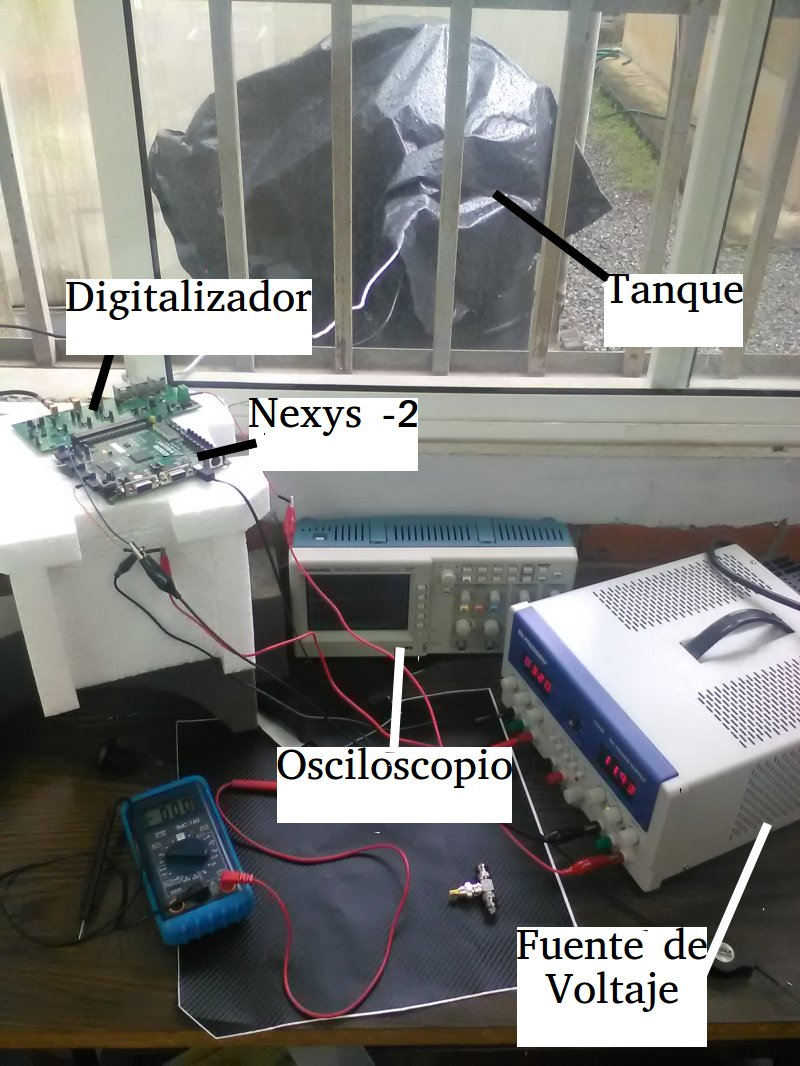
\includegraphics[width = 0.5\linewidth]{ConfiguracionFinal.jpg}

(Fuente propia)
\caption{Tanque de polietileno, de 600L marca Talishte utilizado como base del detector}
\end{center}
\end{figure}

\section{Calibraci\'on por histograma de datos de Kinich Ahau}
El VEM se determin\'o a partir de los histogramas de carga integrada obtenidos de los programas "cal.cc" de ACQUA aplicados a datos crudos obtenidos de "raw.cc" de ACQUA. El valor de VEM es el de la de carga integrada (medida en ADCq) que corresponde al segundo m\'aximo del histograma generado por los datos de carga integrada en los archivos de salida de cal.cc. Este m\'aximo, a su vez, corresponde a la energ\'ia de un mu\'on vertical.

Para la calibraci\'on, se sigui\'o el procedimiento descrito en \citep{ALLISON}. Luego de obtener el valor VEM, se clasificaron los eventos del experimento en dos: a) eventos separados del evento anterior por 1 a 3 $\mu$s y b) eventos separados del anterior entre 8 a 11 $\mu$s. La separaci\'on de tiempo del primer tipo de eventos est\'a centrada en el valor de la vida media del mu\'on, por lo que estos eventos correponder\'ian a muones que decaen. La segunda clasificaci\'on recoge muones que atraviesan el tanque (no decaen). Las posiciones en ADCq de los m\'aximos de cada histograma se compararon para concluir si son iguales o hay diferencias. El valor en VEM del primer m\'aximo se compar\'o con el cociente entre los pulsos caracter\'isticos integrados del mu\'on y electr\'on de Michael generados en la simulaci\'on.

%%%%%%%%%%%%%%%%Cap\'itulo nuevo

\Chapter{Resultados y discusi\'on}

\section{Pulsos caracter\'isticos de part\'iculas incidentes por simulaci\'on}

Se calcularon los pulsos para 1000 eventos de muones, 500 eventos de part\'iculas gamma de 100MeV y 500 eventos de electrones de 37MeV. Las gr\'aficas de los 2000 pulsos se pueden encontrar en la secci\'on de anexos. El valor p de la prueba Shapiro de la distribuci\'on de la amplitud en cada tiempo hizo descartar que las distribuciones fueran normales. Sin embargo, el c\'alculo del intervalo de confianza es robusto ante el supuesto de normalidad. La forma caracter\'istica del pulso de cada tipo de part\'icula dada por el promedio de cada amplitud se ilustra en la figura 7.1.

\begin{figure}[h] %opci\'on h - here pone la imagen aqu\'i en esta posici\'on del documento
\begin{center}
 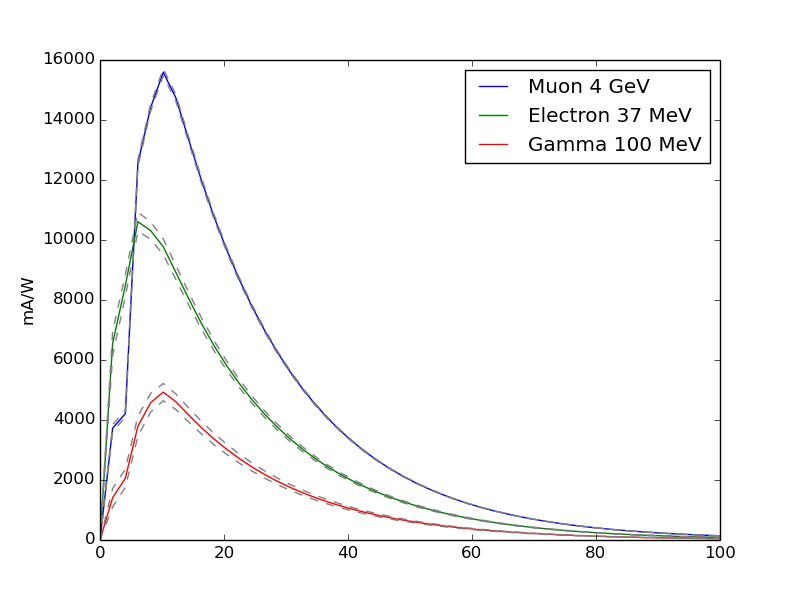
\includegraphics[width=\linewidth]{PulsosCaracteristicos.png}
\caption{El promedio de todos los pulsos para cada tipo de part\'icula}
\end{center}
\end{figure}

El \'area bajo estas curvas representa una medida proporcional a la carga integrada que se obtiene del experimento con el WCD. Por lo tanto, tomando al pulso caracter\'istico del mu\'on de 4GeV (que atraviesa el tanque), se obtiene una definici\'on an\'aloga de $VEM_s$ en t\'erminos de la respuesta inmediata del fotoc\'atodo (en $mA$). La utilidad de esto es que se pueden expresar las cargas integradas del electr\'on de 37 MeV y de part\'iculas gamma en t\'erminos de esta definici\'on de $VEM_s$. Calculando el \'area del pulso del mu\'on con el m\'etodo de trapecio, se define entonces $VEM_s \equiv 123813 mA\times s$. Las \'areas del electr\'on de Michael y de la part\'icula gamma de 100MeV ser\'ian $0.680542 VEM_s$ y $0.317576 VEM_s$. Estos valores pueden ubicarse en los histogramas de carga obtenidos de una corrida de Kinich Ahau luego de haber definido el VEM del tanque.

El cuadro 7.1 y la figura 7.2 exponen los resultados de analizar la amplitud m\'axima (valor discreto m\'as grande en los datos) y tiempo de subida (tiempo en que la se\~nal toma desde 0\% hasta su amplitud m\'axima) para los pulsos generados de cada part\'icula en la simulaci\'on. Estos resultados de la simulaci\'on se comparan con los obtenidos por Miguel Novella para el presente megaproyecto, quien desarroll\'o este an\'alisis para los datos del experimento.

\begin{table}[h]
\caption{ Intervalos de confianza para los valores medios de amplitud y tiempo de subida para cada tipo de part\'icula incidente}
\centering
\begin{tabular}{l | c c}
\hline
Tipo de part\'icula & Amplitud (A/W) & Tiempo de subida (ns) \\ \hline
Mu\'on vertical 4GeV & (15.5, 15.9) & (10.15, 10.19) \\
Electr\'on de Michael 37MeV & (10.5,11.9) & (6.63, 6.94) \\
Part\'icula Gamma 100 MeV & (4.5, 6.0) & (8.66, 9.19)\\

\hline
\end{tabular}
\end{table}

\begin{figure}[h] %opci\'on h - here pone la imagen aqu\'i en esta posici\'on del documento
\begin{center}
 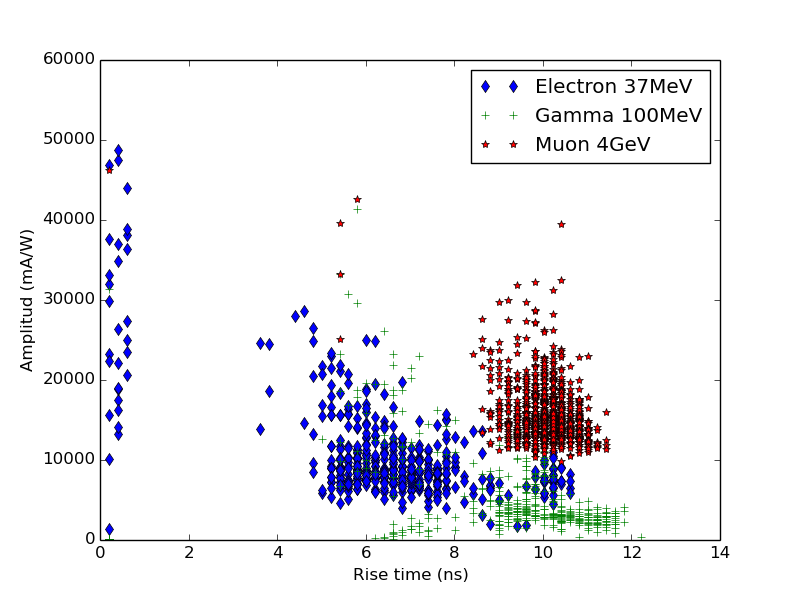
\includegraphics[width=\linewidth]{RiseTimeAmp.png}
\caption{Representaci\'on gr\'afica de la relaci\'on entre amplitud y tiempo de subida para los diferentes tipos de part\'iculas que generaron los pulsos en la simulaci\'on}
\end{center}
\end{figure}

Dado que los intervalos de confianza de amplitudes entre los tres tipos de part\'iculas no coinciden, se acepta la hip\'otesis alterna de que las amplitudes de los pulsos son diferentes. Esto es bastante claro a partir de la figura 7.1 pero vale la pena resaltar. De manera an\'aloga, se acepta la hip\'otesis alterna de que los tiempo de subida son diferentes para cada pulso.

La gr\'afica 7.2 se realiz\'o para evidenciar que las relaciones entre amplitud y tiempo de subida para cada pulso son diferentes entre s\'i. Los puntos rojos se ubican en una regi\'on diferente en el plano que los puntos azules. Esta distinci\'on se puede comparar con el experimento con el tanque, ya que el modo de calibraci\'on de histograma permiti\'o la clasificaci\'on de tipos de eventos de manera independiente. Por otro lado, la figura 7.2 muestra cierta correspondencia con la referida en la figura 5.8 de la secci\'on 5.3.1. La diferencia m\'as importante es la escala de tiempo de subida: mientras que los electrones en la simulaci\'on tuvieron tiempos de subida centrados alrededor de (6.63, 6.94)ns, los de \citep{Salazar} lo est\'an alrededor de los 10ns, y la diferencia es a\'un mayor para los muones. Sin embargo, esto podr\'ia explicarse por la diferencia en las dimensiones del tanque: el utilizado en \citep{Salazar} ten\'ia un di\'ametro de 1.54 m mientras que Kinich Ahau tiene un di\'ametro de 0.42 m, ambos con el mismo alto.

\section{N\'umero de fotones prodcidos y detectados con un mu\'on que atraviesa en la simulaci\'on}

La cantidad de fotones producidos por muones que entran al tanque es proporcional principalmente a la distancia que recorre en el tanque cuando los  muones no decaen. En esta secci\'on se investiga tambi\'en la dependencia de los fotones producidos y detectados sobre la energ\'ia de los muones incidentes para eventos en la simulaci\'on.

Primero se investig\'o la normalidad de los fotones producidos, detectados y el cociente de estos valores para el evento de un mu\'on vertical de 4GeV. Los detalles de este an\'alisis se encuentran en anexos. Se compararon las cantidades de fotones detectados para diferentes energ\'ias de muones verticales. Esto para poner a prueba las hip\'otesis:

\begin{itemize}
\item $H_4o$: No hay relaci\'on entre la energ\'ia de un muon vertical que atraviesa y el n\'umero de fotones detectados.
\item $H_4a$: Hay relaci\'on entre la energ\'ia de un muon vertical que atraviesa y el n\'umero de fotones detectados
\end{itemize}

El an\'alisis de la normalidad de las distribuciones revela que la distribuci\'on de los fotones detectados para una energ\'ia no sigue una distribuci\'on normal, sin embargo, el an\'alisis ANOVA para la diferencia de dos medias es robusto ante la suposici\'on de normalidad, en especial porque el tama\~no muestral es grande (n=1000 o 500). Por lo tanto, se prosigi\'o a calcular la media de fotones detectados para diferentes energ\'ias. Su representaci\'on gr\'afica se muestra en la figura 7.3.

\begin{figure}[h] %opci\'on h - here pone la imagen aqu\'i en esta posici\'on del documento
\begin{center}
 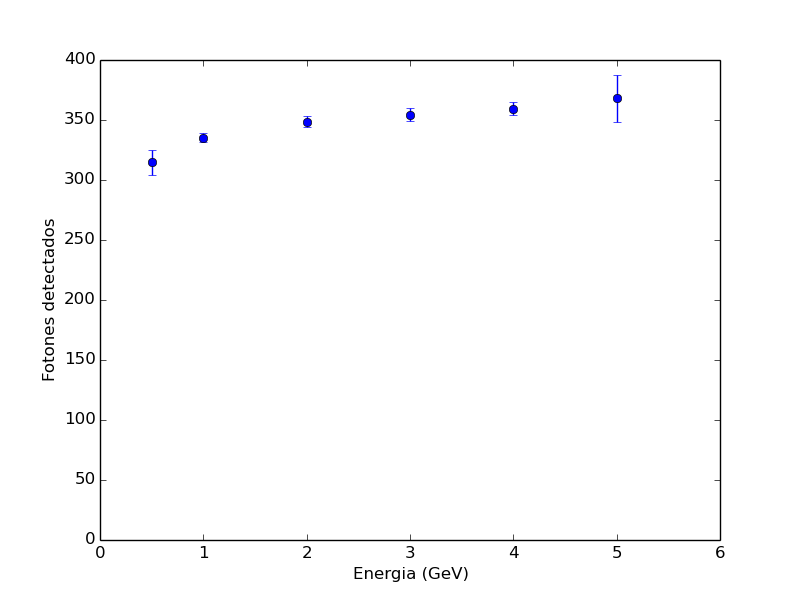
\includegraphics[width=\linewidth]{DetectadosVsEnergia.png}
\caption{Promedio del n\'umero de fotones detectados respecto a la energ\'ia del mu\'on vertical incidente. Las barras de error representan el intervalo de un 95\% de confianza}
\end{center}
\end{figure}

\begin{table}[h]
\centering
\caption{ Resultados de la regresi\'on lineal de los valores del promedio de fotones detectados respecto a energ\'ia de mu\'on vertical incidente}
\begin{tabular}{l | c}
\hline
Pendiente & 10.3 $(GeV)^{-1}$ \\
Intercepto & 320 \\
Coeficiente de correlaci\'on ($r^2$) & 0.876 \\
Valor p & 0.006006693 \\

\hline
\end{tabular}
\end{table}

Debido a que el valor p es menor a $\alpha=0.05$, se acepta la hip\'otesis alterna con un 95\% de confianza. Es decir, el n\'umero de fotones, y por lo tanto, carga integrada, depende de la energ\'ia del mu\'on incidente que atraviesa el tanque incluso si este atraviesa por completo el tanque. Sin embargo, esta dependencia parece ser suficientemente peque\~na (10.3 fotones adicionales por GeV extra del mu\'on), lo que es consistente con las observaciones en \citep{ASOREY} de que el poder de frenado para muones es peque\~no. A\'un as\'i, resultado evidencia que el valor del VEM no solo depende de la geometr\'ia del detector sino que tambi\'en est\'a relacionado con el espectro de energ\'ia de muones incidentes.

\section{Calibraci\'on de Kinich Ahau}
Se capturaron datos durante 4 horas con el tanque Kinich Ahau. Primero se utiliz\'o la extenci\'on -c del archivo "raw.cc" para obtener las cargas integradas de todos los pulsos. Luego, se graficaron estas cargas integradas en forma de histograma. La posici\'on del segundo m\'aximo corresponde a la carga integrada generada por un mu\'on vertical, ya que la direcci\'on de los muones que inciden provenientes de cascadas de \'area extensa sigan una distribuci\'on dada por $\cos^2(\theta)$, donde $\theta$ es el \'angulo medido respecto a la vertical y cuyo valor esperado es justo en $\theta=0$. Se realiz\'o una regresi\'on cuadr\'atica en el intervalo [140,240]ADCq (escogido visualmente) y se determin\'o el valor del VEM de $190 \pm 20$. De la misma manera, se obtuvo el punto de transici\'on (el valor m\'inimo antes del VEM) de $101\pm20$.

\begin{figure}[h] %opci\'on h - here pone la imagen aqu\'i en esta posici\'on del documento
\begin{center}
 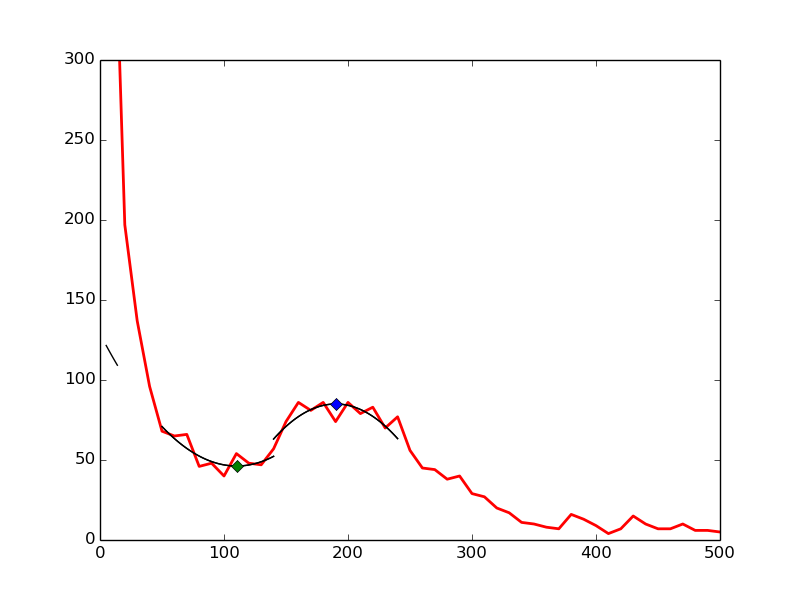
\includegraphics[width=0.7\linewidth]{ADCqCorrida1.png}
\caption{Histogramas ADCq de 4 horas de funcionamiento del detector, con el segundo pico identificado con una regresi\'on cuadr\'atica entre 140 ADCq y 240 ADCq y el punto de transici\'on con el mismo m\'etodo entre 50ADCq y 140 ADCq}
\end{center}
\end{figure}

No existe un primer pico para los eventos de la banda electrom\'agnetica debido a que estos son los datos crudos, que incluyen todo el posible ruido de \textit{afterpulses}. Usando el valor de VEM, se clasificaron los eventos por bandas de acuerdo al modo histograma. El valor m\'aximo de muones que cruzan corresponde a la diagonal en el tanque. Usando las dimensiones de Kinich Ahau ($114\pm1$ cm de altura y $41\pm1$ cm de di\'ametro), se obtiene un valor de carga m\'axima por muones que cruzan de $1.06\pm0.04$ VEM, o $201\pm7$ ADCq. Este valor no es diferente al encontrado para el VEM, lo que se puede interpretar como el hecho de que no hay diferencia apreciable entre la carga integrada por muones verticales (que atraviesan $114\pm1$ cm) y muones diagonales (que atraviesan $121\pm4$ cm).

Por otro lado, se realiz\'o otra clasificaci\'on de eventos de acuerdo a lo descrito en metodolog\'ia: eventos cuya diferencia de tiempo con el anterior fue entre 1$\mu$s y 3 $\mu$s y eventos entre 8 $\mu$ y 11 $\mu$. Los datos clasificados se tomaron directamente de los archivos generados por "raw.cc" de ACQUA. A partir de ellos, se generaron dos archivos con todos los pulsos que califican seg\'un la clasificaci\'on, respectivamente. Los archivos registran por fila el valor de carga integrada de cada pulso. Se generaron histogramas de carga para cada clasificaci\'on de eventos, dados en la figura 7.5. Los programas que se utilizaron para la clasificaci\'on y la generaci\'on de histogramas fueron desarrollados por Miguel Novella para el presente megaproyecto, y est\'an descritos en la secci\'on de anexos.

\begin{figure}[h] %opci\'on h - here pone la imagen aqu\'i en esta posici\'on del documento
\begin{center}
 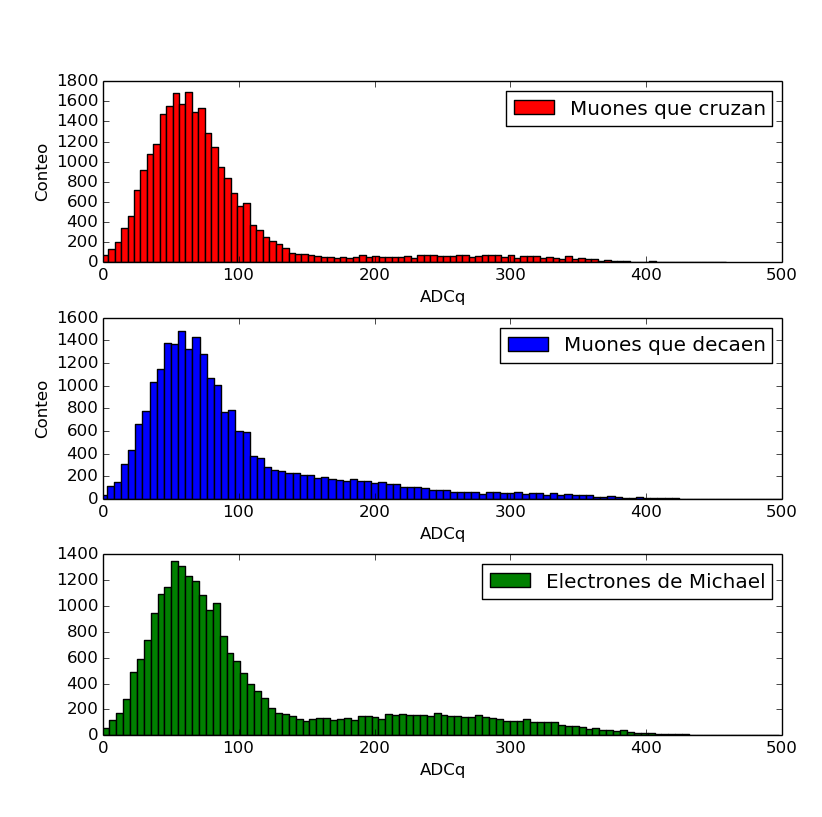
\includegraphics[width=0.9\linewidth]{HistogramasAll.png}
\caption{Histogramas ADCq de 4 horas de funcionamiento del detector para a) eventos con diferencia de 8 a 11 $\mu$s del anterior que corresponden a muones que cruzan el tanque, b) primero de los eventos con diferencia de 1 a 3 $\mu$s que corresponden a muones que decaen y c) segundo de los eventos con diferencia de 1 a 3 $\mu$s que corresponden a electrones de Michael}
\end{center}
\end{figure}

Las posiciones de los picos se encontraron con regresiones polinomiales alrededor de 0-100 ADCq para el primer pico y 200-300 ADCq para el segundo pico. Los resultados se resumen en el cuadro 7.3, y el programa que se utiliz\'o se puede encontrar en la secci\'on 9.8 del cap\'itulo Anexos.

%\pagebreak
\begin{table}[h]
\caption{ Posici\'on de los picos de los histogramas de muones que cruzan, muones que decaen y electrones de Michael, encontrados con regresiones cuadr\'aticas alrededor de los picos}
\centering
\begin{tabular}{l | c c}
\hline
Histograma & Primer pico (ADCq) & Segundo pico (ADCq) \\ \hline
Muones que cruzan & 57 $\pm$ 8 & 260 $\pm$ 20 \\
Muones que decaen & 58 $\pm$ 5 & 331 $\pm$ 182 \\
Electrones de Michael & 57 $\pm$ 7 & 231 $\pm$ 20\\ \hline
Promedio & 58 $\pm$ 7 & 250 $\pm$ 20*\\

\hline
\end{tabular}\\
* No se tom\'o en cuenta el segundo pico del segundo histograma\end{table}

La posici\'on del segundo pico en el histograma de muones que decaen tiene una incertidumbre mayor al intervalo sobre el que se busc\'o; evidentemente a partir de la figura 7.4 tambi\'en se ve observa que este segundo pico no aparece. Esto quiere decir que el criterio de clasificaci\'on para los eventos de este histograma parece excluir por completo eventos de muones que atraviesan el tanque.

El valor de VEM para Kinich Ahau obtenido del segundo m\'aximo de estos histogramas es de $230 \pm 20$. Este valor es diferente al obtenido en la gr\'afica de la figura 7.4. Se utiliza el valor obtenido en el cuadro 7.3 como valor del VEM ya que la ausencia del m\'aximo VEM para los eventos de muones que decayeron da confianza de que los m\'aximos en el histograma de muones que atraviesan s\'i es de muones que atraviesan por completo el tanque. Con este valor, se clasificaron los eventos por bandas de acuerdo al modo histograma.

El valor del primer pico expresado en unidades del VEM ser\'ia $0.232 \pm 0.019$ VEM. Las integrales de los pulsos caracter\'isticos del mu\'on que atraviesa y el electr\'on de Michael de la simulaci\'on son $VEM_s \equiv 123813 mA\times s$ y 84260 $mA\times s$, respectivamente. El segundo, expresado en el valor definido $VEM_s$ es $0.680542 VEM_s$; este n\'umero deber\'ia de ser equivalente al valor en VEM del primer pico de los hisgoramas de la figura 7.4. Estos valores no coinciden, lo que es evidencia de que el primer pico de los histogramas no corresponde a la energ\'ia de electrones de Michael.

%%%%%%%%%%%%%%%%Cap\'itulo nuevo

\Chapter{Conclusiones}

Se caracteriz\'o las se\~nales de pulsos t\'ipicos del experimento, obteniendo las amplitudes y tiempos de subida promedio de tres tipos de evento: muones de 4GeV que logran atravesar el tanque, part\'iculas gamma de 100 MeV que producen pares cargados y electrones con energ\'ias t\'ipicas de la distribuci\'on de Michael en el decaimiento de un mu\'on. La relaci\'on entre amplitud y tiempo de subida muestra correspondencia con la referencia utilizada, y se encontr\'o que es posible identificar part\'iculas utilizando este par\'ametro porque los promedios de cada uno son distintos entre s\'i.

Se encontr\'o tambi\'en que la cantidad de fotones detectados en la simulaci\'on por muones con energ\'ias suficientes para atravesar el tanque depende de la energ\'ia de los muones, con una correlaci\'on de 10.3 $GeV^{-1}$ y un valor p de 0.006 para la regresi\'on lineal. Este valor es peque\~no, y es consistente con las observaciones de que el poder de frenado de los muones en agua es suficientemente bajo para considerar que todos los muones verticales depositan aproximadamente la misma energ\'ia en un WCD.

Se encontr\'o el valor VEM para todos los pulsos de una corrida de 4 horas de Kinich Ahau, de (190 $\pm$ 20) ADCq, mientras que el mismo procedimiento realizado para eventos separados entre 8-11 y 1-3 microsegundos entre s\'i resulta en un valor de (250 $\pm$ 20) ADCq. Se utiliza el segundo valor ya que la ausencia del m\'aximo VEM para los eventos de muones que decayeron da confianza de que los m\'aximos en el histograma de muones que atraviesan s\'i es de muones que atraviesan por completo el tanque. El valor m\'aximo en los histogramas de carga  de los eventos clasificados para la banda electromagn\'etica es $0.232 \pm 0.019$ VEM que no coincide con el valor $0.680542$ $VEM_s$ de la simulaci\'on de electrones de 37 MeV de energ\'ia, lo que es evidencia de que el primer pico de los histogramas no corresponde a la energ\'ia de electrones de Michael.

% % % % % % % % % % % % % % % % % % % % % % %                       Secci\'on de bibliograf\'ia

\Biblio
\begin{thebibliography}{9}
\Bibliotoc
\bibitem[Alarc\'on, M. et al (1999)]{ALARCON} Alarc\'on, M. et al. 1999. \textit{Calibration and monitoring of water Cherenkov detectors with stopping and crossing muons}. Nuclear Instruments and Methods in Physics. Research A 420: 39-47. Disponible en: http://www.ung.si/public/pao/bibl/nim\_420\_ma.pdf [con acceso el 16 de noviembre del 2015]

\bibitem[Allison, P. et al. (2005)]{ALLISON} Allison, P. et al. 2005. \textit{Observing muon decays in water Cherenkov detectors at Pierre Auger Observatory}. 29th International Cosmic Ray Conference Pune 00, 101-104. Disponible en: http://arxiv.org/pdf/astro-ph/0509238.pdf [tomado el 16 de noviembre del 2015]


\bibitem[Asorey, H. (2012)]{ASOREY} Asorey, H. 2012. \textit{Los detectores Cherenkov del observatorio Pierre Auger y su aplicaci\'on al estudio de fondos de radiaci\'on}. Tesis Universidad Nacional de Cuyo. 286 p\'aginas.

\bibitem[Asorey, H. y S. Dasso (2015)]{ASOREY2015} Asorey, H. y S. Dasso. 2015. \textit{LAGO: the Latin American Giant Observatory}. The 34th International Cosmic Ray Conference. The Hague, Pa\'ses Bajos.

\bibitem[Arnaldi, H. (2011)]{ARNALDI} Arnaldi, H. 2011. \textit{Interfaces LAGO}, Laboratorio de Detecci\'n de Part\'iculas y Radiaci\'on, Centro At\'omico Bariloche.

\bibitem[Baldini, L. (2014)]{BALDINI} Baldini, L. 2014 \textit{Space-Based Cosmic-Ray and Gamma-Ray Detectors: a Review}. Universidad de Pisa. Disponible en: https://arxiv.org/pdf/1407.7631v2.pdf [con acceso el 24 de octubre del 2016

\bibitem[Bernlohr, K. (2015)]{BERN} Bernlohr, K. 2015. \textit{Cosmic Ray / Gamma ray / Neutrino and similar experiments}. Disponible en: https://www.mpi-hd.mpg.de/hfm/CosmicRay/CosmicRaySites.html\#cosmic-ray+gamma-ray [con acceso el 24 de octubre del 2016

\bibitem[Calderon, R., H. Asorey y L. N\'u\~nez (2005)]{CALDERON} Calderon, R, H. Asorey y L. N\'u\~nez \textit{Geant4 based simulation of the Water Cherenkov Detectors of the LAGO project}. Disponible en: http://arxiv.org/pdf/1503.07270.pdf [consultado el 4 de julio 2016]

\bibitem[Chen, M. et al. (2006)]{CHEN} Chen, M. et al. 2006. \textit{A study of the water Cherenkov calorimeter}. Preimpresi\'on presentada a Eliver Science. Disponible en: http://arxiv.org/pdf/physics/0602169.pdf [consultado el 15 de marzo del 2016]

\bibitem[Cherenkov, P. (1958)]{CHERENKOV} Cherenkov, P. 1958. \textit{Radiation of particles moving at a velocity exceeding that of light, and some of the possibilities for their use in experimental physics}. Nobel Lecture. P. 15.

\bibitem[Dasso, S. y H. Assorey (2012)]{DASSO} Dasso, S. y H. Assorey. 2012. {\title The Scaler Mode in Pierre Auger Observatory to study heliospheric modulations of cosmic rays}. arXiv:1204.6196

\bibitem[DuPont. (2009)]{DUPONT} Dupont. 2009. \textit{Material Safety Data Sheet: DuPont Tyvek ® Spundbond Polyethyene}. Estados Unidos. Disponible en: http://www.dupont.com/content/dam/assets/products-and-services/construction-materials/assets/DuPont\_Tyvek\_Spunbond\_Polyethylene\_MSDS\_2009-04-21.pdf 

\bibitem[Geant4 User's Guide (2015)]{GEANT4} Geant4. 2015. \textit{Geant4 User's Guide – For Application Developers -}. Disponible en:\\ http://geant4.web.cern.ch/geant4/G4UsersDocuments/UsersGuides/ForApplicationDeveloper\\/html/index.html [consultado el 15 de mayo del 2016]

\bibitem[Grupen, C y B. Shwartz (2008)]{GROUPENS} Grupen, C y B. Shwartz. 2008  \textit{Particle Detectors}. Segunda edici\'on. Cambridge University Press, Reino Unido.

\bibitem[Guan et al. (2006)]{GUAN} Guan, M. et al. 2006.  \textit{Muon Simulation at the Daya Bay site}. Disponible en: \\http://www.osti.gov/scitech/servlets/purl/1006397 [con acceso el 17 de octubre del 2016]

\bibitem[Gumplinger (2002)]{GUMP} Gumplinger, P. 2002.  \textit{Optical Photon Processes in GEANT4}. Users' Workshop en SLAC, Universidad de Stanford. Disponible en: http://geant4.slac.stanford.edu/UsersWorkshop/PDF/Peter/OpticalPhoton.pdf [con acceso el 19 de octubre del 2016]

\bibitem[Hamamatsu (2007)]{Hamamatsu} Hamamatsu. 2007.  \textit{Photomultiplier Tubes Basics and Applications}. Tercera edici\'on. Disponible en: https://www.hamamatsu.com/resources/pdf/etd/PMT\_handbook\_v3aE.pdf [con acceso el 19 de octubre del 2016]

\bibitem[Heck, D. et al (1998)]{HECK} Heck, D. 1998. \textit{CORSIKA: A Monte Carlo code to simulate Extensive Air Showers}. Disponible en: https://web.ikp.kit.edu/corsika/physics\_description/corsika\_phys.pdf [con acceso el 18 de marzo del 2016]

\bibitem[Hoover, S. et al (2010)]{HOOVER} Hoover, S. et al. 2010. \textit{Observation of ultra-high-energy Cosmic Rays with the ANITA Balloon-borne Radio Interferometer}. Disponible en: https://arxiv.org/pdf/1005.0035v2.pdf [con acceso el 24 de octubre del 2016]

\bibitem[Lukens, J., B. Reid y A. Tuggle (2010)]{LUKENS} Lukens, J., B. Reid y A. Tuggle.  2010. \textit{Experiment in muon Decay}. Universidad de Alabama.

\bibitem[Nielsen, C. (2010)]{NIELSEN} Nielsen, C.  2010. \textit{Calibration Through Simulation of a Low-Energy Cherenkov Detector}. Tesis University of California, Santa Barbara. Disponible en: http://www.physics.ucsb.edu/sites\\/secure.lsit.ucsb.edu.phys.d7/files/sitefiles/education/ Nielsen.pdf [con acceso el 2 de junio del 2016]

\bibitem[P\'erez, Y. (2009)]{PEREZ} P\'erez, Y. 2009. \textit{Caracterizaci\'on de Detectores Cherenkov en el Proyecto LAGO}. Trabajo especial de grado. Universidad de los Andes.

\bibitem[P\'erez, Y. (2015)]{YUNIOR} P\'erez, Y. 2015. \textit{Aplicaci\'on en meteorolog\'ia espacial de los datos del proyecto LAGO (Latin American Giant Observatory)}. Tesis de postgrado. Universidad de los Andes.

\bibitem[Photonis (SF)]{Photonis} Photonis. (SF). \textit{Photomultiplier XP1802 Datasheet}. Disponible en: http://www.qsl.net/k0ff/016\%20Manuals/PMT/Photonis/XP1802.pdf [con acceso el 2 de octubre del 2016]

\bibitem[Seo, E. et al (2004)]{SEO} Seo, E. et al. 2004. \textit{Cosmis-ray energetics and mass (CREAM) balloon project}. Advances in Space Research 33. Disponible en: http://cosmicray.umd.edu/cream/images/stories/files/frontpage/seo.pdf [con acceso el 24 de octubre del 2016]

\bibitem[Salazar, H. y L. Villase\~nor (2005)]{Salazar} Salazar, H. y L. Villase\~nor (2005) \textit{Cosmis-ray energetics and mass (CREAM) balloon project}. Advances in Space Research 33. Disponible en: http://cosmicray.umd.edu/cream/images/stories/files/frontpage/seo.pdf [con acceso el 24 de octubre del 2016]

\bibitem[Sofo, M. (2011)]{SOFO} Sofo, M. 2011. \textit{Electr\'onica LAGO: Gu\'ia de conexi\'on de Hardware}, Laboratorio de Detecci\'n de Part\'iculas y Radiaci\'on, Centro At\'omico Bariloche.

\bibitem[Suarez (2014)]{SUAREZ} Suarez, M. 2014. \textit{Seminario Cascadas A\'ereas Extensas (EAS) para la colaboraci\'on LAGO, Sesi\'on 2}. Disponible en: https://www.youtube.com/watch?v=AP9i5pdbJNc [con acceso el 2 de septiembre del 2015]

\bibitem[Villase\~nor et al (2011)]{VILLASENOR} Villase\~nor, L. y et al. 2011. \textit{Search for Gamma Ray Bursts and Forbush Decreases in the LAGO Observatory}. International Cosmic Ray Conference, Beijing. $(10)$: 314.

\bibitem[Watson, A (2002)]{WATSON} Watson, A. 2002. \textit{Extensive Air Shower and Ultra High Energy Cosmic Rays}. Disponible en: http://www.ast.leeds.ac.uk/Auger/augerthesis/mexlects3.pdf [con acceso el 21 de octubre del 2016]

% \bibitem[Como aparece al citar]{referencia} Datos Bibliogr\'aficos

\end{thebibliography}



 % % % % % % % % % % % % % % % % % % % % % %                                   Ap\'endices

\Chapter{Anexos}

\section{M\'as detalle de la geometr\'ia en la simulaci\'on}
\begin{table}[h]
\caption{ Descripci\'on de los objetos en la simulaci\'on y sus jerarqu\'ias l\'ogicas}
\centering
\begin{tabular}{l c c c c }
\hline
Nombre & \specialcell{Volumen madre\\(posici\'on)} & Material & Tipo & Dimensiones  \\

 \hline
\hline
World & ninguno & Aire & G4Box & 1 metro por lado\\ \hline
Tyvek & \specialcell{World\\(0,0,0)} & Tyvek & G4Cons & \specialcell{Radio interno a = 0m\\Radio interno b = 0m\\ Radio externo a = 40.1m\\Radio externo b = 40.1m\\Altura = 57.1cm\\\'Angulo m\'inimo = $0^o$\\\'Angulo m\'aximo = $360^o$}\\ \hline
Agua & \specialcell{Tyvek\\(0,0,0)} & Agua & G4Cons & \specialcell{Radio interno a = 0m\\Radio interno b = 0m\\ Radio externo a = 40.0m\\Radio externo b = 40.0m\\Altura = 57.0cm\\\'Angulo m\'inimo = $0^o$\\\'Angulo m\'aximo = $360^o$}\\ \hline
Vidrio PMT & \specialcell{Agua\\(0,0,57cm)} & Borosilicato & G4Sphere & \specialcell{Radio interno = 0.0m\\Radio externo = 11.4cm\\\'Angulo $\phi$ m\'inimo = $0^o$\\\'Angulo $\phi$ que abarca = $360^o$\\\'Angulo $\theta$ m\'inimo = $0^o$\\\'Angulo $\theta$ que abarca = $360^o$}\\ \hline
Fotoc\'atodo PMT & \specialcell{Vidrio PMT\\(0,0,0)} & Aluminio & G4Sphere & \specialcell{Radio interno = 0.0m\\Radio externo = 11.1cm\\\'Angulo $\phi$ m\'inimo = $0^o$\\\'Angulo $\phi$ que abarca = $360^o$\\\'Angulo $\theta$ m\'inimo = $0^o$\\\'Angulo $\theta$ que abarca = $360^o$}\\ \hline
Vac\'io dentro PMT & \specialcell{Fotoc\'atodo PMT\\(0,0,0)} & Vac\'io & G4Sphere & \specialcell{Radio interno = 0.0m\\Radio externo = 11.0cm\\\'Angulo $\phi$ m\'inimo = $0^o$\\\'Angulo $\phi$ que abarca = $360^o$\\\'Angulo $\theta$ m\'inimo = $0^o$\\\'Angulo $\theta$ que abarca = $360^o$}\\ \hline
\hline
\end{tabular}
\end{table}

\begin{table}[h]
\caption{ Propiedades de material asignadas al agua en la simulaci\'on a trav\'es de la clase G4MaterialsPropertiesTable y asignadas a 32 energ\'ias de fot\'on}
\centering
\begin{tabular}{c c c | c c c}
\hline
\specialcell{Energ\'ia\\del fot\'on (eV)} & \specialcell{\'Indice de\\refracci\'on} & \specialcell{Largo de\\atenuaci\'on (m)} & \specialcell{Energ\'ia\\del fot\'on (eV)} & \specialcell{\'Indice de\\refracci\'on} & \specialcell{Largo de\\atenuaci\'on (m)} \\
2.034                     & 1.3435                   & 3.448                     & 2.757                     & 1.3522                   & 55.556                    \\
2.068                     & 1.344                    & 4.082                     & 2.82                      & 1.353                    & 52.632                    \\
2.103                     & 1.3445                   & 6.329                     & 2.885                     & 1.3535                   & 52.632                    \\
2.139                     & 1.345                    & 9.174                     & 2.954                     & 1.354                    & 47.619                    \\
2.177                     & 1.3455                   & 12.346                    & 3.026                     & 1.3545                   & 45.455                    \\
2.216                     & 1.346                    & 13.889                    & 3.102                     & 1.355                    & 41.667                    \\
2.256                     & 1.3465                   & 15.152                    & 3.181                     & 1.3555                   & 37.037                    \\
2.298                     & 1.347                    & 17.241                    & 3.265                     & 1.356                    & 33.333                    \\
2.341                     & 1.3475                   & 18.868                    & 3.353                     & 1.3568                   & 30                        \\
2.386                     & 1.348                    & 20                        & 3.446                     & 1.3572                   & 28.5                      \\
2.433                     & 1.3485                   & 26.316                    & 3.545                     & 1.358                    & 27                        \\
2.481                     & 1.3492                   & 35.714                    & 3.649                     & 1.3585                   & 24.5                      \\
2.532                     & 1.35                     & 45.455                    & 3.76                      & 1.359                    & 22                        \\
2.585                     & 1.3505                   & 47.619                    & 3.877                     & 1.3595                   & 19.5                      \\
2.64                      & 1.351                    & 52.632                    & 4.002                     & 1.36                     & 17.5                      \\
2.697                     & 1.3518                   & 52.632                    & 4.136                     & 1.3608                   & 14.5 \\

 \hline
\hline

\hline
\end{tabular}
\end{table}

\pagebreak
\section{Programa utilizado para las distribuciones de fotones producidos, detectados y su cociente en la simulaci\'on}

\lstinputlisting[language=bash]{DistFotonesPres.py}

\pagebreak
\section{Normalidad de fotones producidos y detectados en la simulaci\'on}

\begin{figure}[h] %opci\'on h - here pone la imagen aqu\'i en esta posici\'on del documento
\begin{center}
 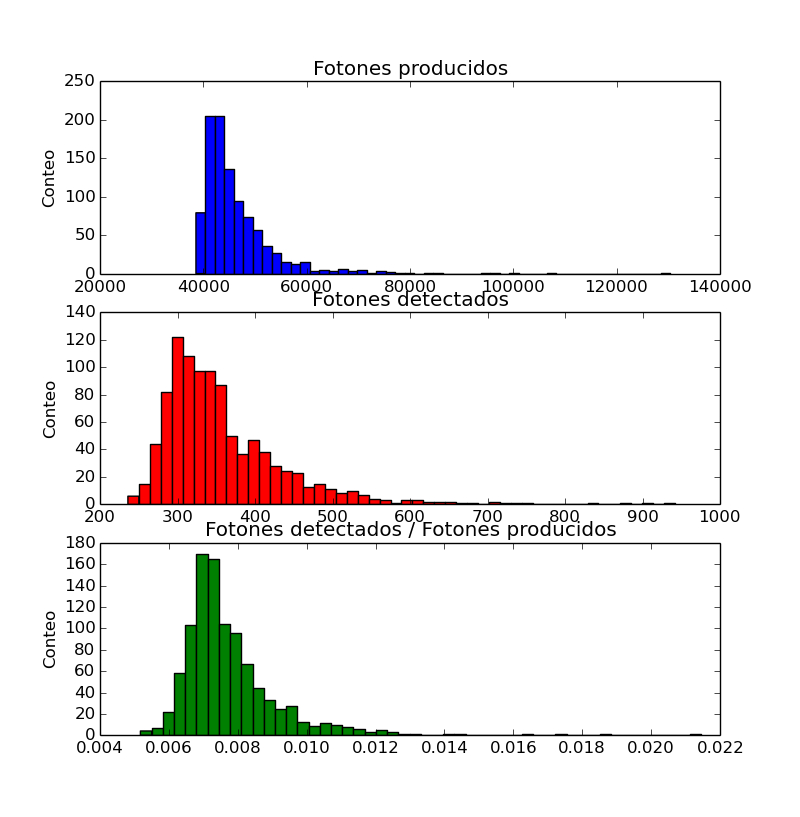
\includegraphics[width=0.8\linewidth]{FotonesMuonVerticalG4.png}
\caption{Histogramas de los fotones producidos, fotones detectados y el cociente de los fotones detectados sobre los producidos para un mu\'on vertical de 4GeV en la simulaci\'on, con un tama\~no muestral de 1000 eventos}
\end{center}
\end{figure}

Los histogramas en la figura 7.1 sugieren que las distribuciones no siguen una distribuci\'on normal. Como complemento se us\'o la prueba Shapiro-Wilk para las hip\'otesis:

Fotones producidos
\begin{itemize}
\item $H_1o$: La distribuci\'on de fotones producidos para el evento de un mu\'on vertical tiene normalidad
\item $H_1a$: La distribuci\'on de fotones producidos para el evento de un mu\'on vertical no tiene normalidad
\end{itemize}

Fotones detectados
\begin{itemize}
\item $H_2o$: La distribuci\'on de fotones detectados para el evento de un mu\'on vertical tiene normalidad
\item $H_2a$: La distribuci\'on de fotones detectados para el evento de un mu\'on vertical no tiene normalidad
\end{itemize}

Cociente de fotones detectados sobre fotones producidos
\begin{itemize}
\item $H_3o$: La distribuci\'on del cociente de fotones detectados sobre fotones producidos para el evento de un mu\'on vertical tiene normalidad
\item $H_3a$: La distribuci\'on del cociente de fotones detectados sobre fotones producidos para el evento de un mu\'on vertical no tiene normalidad
\end{itemize}

\begin{table}[h]
\caption{ Valores p para la prueba Shapiro-Wilk de normalidad de las distribuciones de los fotones producidos, detectados y el cociente}
\centering
\begin{tabular}{l | c}
\hline
Distribuci\'on & valor p de la prueba \\ \hline
Fotones producidos & 5.922653054979643e-32 \\
Fotones detectados & 1.7184711613370248e-39 \\
$\frac{Fotones detectados}{Fotones producidos}$ & 9.682787576723116e-34 \\

\hline
\end{tabular}
\end{table}

Por los valores dados en el cuadro 7.1 por la prueba Shapiro-Wilk y por la forma de los histogramas en la figura 7.1, se concluye que ninguna de las distribuciones tiene normalidad.

\section{Programa utilizado para la obtenci\'on de los pulsos caracter\'isticos}

\lstinputlisting[language=bash]{PulsosCaract.py}

\pagebreak
\section{Gr\'aficas de los 2000 pulsos analizados para la caracterizaci\'on de la simulaci\'on}

\begin{figure}[h] %opci\'on h - here pone la imagen aqu\'i en esta posici\'on del documento
\begin{center}
 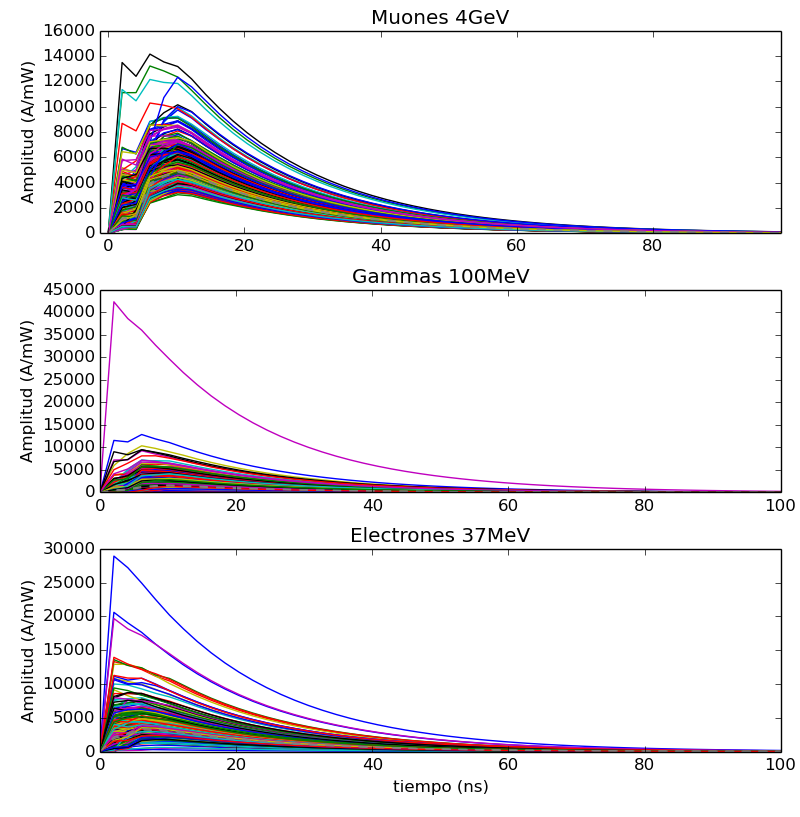
\includegraphics[width=\linewidth]{2000Pulsos.png}
\caption{a) 1000 pulsos sobrepuestos de las detecciones de fotones para mu\'on vertical de 4GeV, b) 500 pulsos sobrepuestos de las detecciones de fotones para part\'iculas gamma de 100 MeV, c) 500 pulsos sobrepuestos de las detecciones de fotones para electr\'on de Michael de 37 MeV}
\end{center}
\end{figure}

\pagebreak
\section{Programa utilizado para el c\'alculo de apmlitudes y tiempo de subida}

\lstinputlisting[language=bash]{VariablesPulsos.py}

\section{Programa utilizado para la clasificaci\'on de muones, desarrollado por Miguel Novella}

\lstinputlisting[language=bash]{clasificadorMuones.py}

\section{Programa utilizado para el c\'alculos de los m\'aximos en los histogramas}

\lstinputlisting[language=bash]{Picos.py}

\end{document}

